\documentclass[11pt]{article}
\usepackage[margin=1in]{geometry}
\usepackage[T1]{fontenc}
\usepackage{mathptmx}
\renewcommand{\ttdefault}{lmtt}
\usepackage{amsmath,amssymb,amsthm}
\usepackage{booktabs,multirow}
\usepackage{graphicx}
\usepackage{enumitem}
\usepackage{xcolor}
\usepackage[numbers,sort&compress]{natbib}
\usepackage[colorlinks,linkcolor=blue!50!black,citecolor=blue!50!black,urlcolor=blue!50!black]{hyperref}
\usepackage{microtype}
\usepackage{tikz}
\usetikzlibrary{positioning,arrows.meta}

\newtheorem{theorem}{Theorem}
\newtheorem{lemma}[theorem]{Lemma}
\newtheorem{proposition}[theorem]{Proposition}
\newtheorem{corollary}[theorem]{Corollary}
\theoremstyle{definition}
\newtheorem{definition}[theorem]{Definition}
\theoremstyle{remark}
\newtheorem{remark}[theorem]{Remark}

\newcommand{\Prob}{\mathbb{P}}
\newcommand{\Comp}{\mathrm{Comp}}
\newcommand{\CP}{\mathrm{CP}^{+}}
\newcommand{\eps}{\varepsilon}
\newcommand{\ind}{\mathbf{1}}
\newcommand{\anp}{\textsc{anp}}

% Replace with the author's name before submission.
\newcommand{\authorname}{dbwls99706}

% Generated by experiments/make_figures.py from results/*.json. Do not edit.
\newcommand{\AbCLevelDeltaLoose}{27.3}
\newcommand{\AbCLevelDeltaStrict}{28.3}
\newcommand{\AbCLevelGridCoarse}{27.8}
\newcommand{\AbCLevelGridDefault}{27.4}
\newcommand{\AbCLevelGridFine}{28.0}
\newcommand{\AbCLevelKnapsack}{27.4}
\newcommand{\AbCLevelPooled}{27.4}
\newcommand{\AbCLevelRefined}{27.4}
\newcommand{\AbCLevelSeparate}{29.2}
\newcommand{\AbCNodeDeltaLoose}{34.0}
\newcommand{\AbCNodeDeltaStrict}{34.8}
\newcommand{\AbCNodeGridCoarse}{32.6}
\newcommand{\AbCNodeGridDefault}{34.0}
\newcommand{\AbCNodeGridFine}{36.8}
\newcommand{\AbCNodeKnapsack}{34.0}
\newcommand{\AbCNodePooled}{34.0}
\newcommand{\AbCNodeRefined}{34.0}
\newcommand{\AbCNodeSeparate}{42.3}
\newcommand{\AbMLevelDeltaLoose}{40.2}
\newcommand{\AbMLevelDeltaStrict}{40.8}
\newcommand{\AbMLevelGridCoarse}{41.0}
\newcommand{\AbMLevelGridDefault}{40.3}
\newcommand{\AbMLevelGridFine}{40.6}
\newcommand{\AbMLevelKnapsack}{40.3}
\newcommand{\AbMLevelPooled}{40.3}
\newcommand{\AbMLevelRefined}{40.3}
\newcommand{\AbMLevelSeparate}{41.5}
\newcommand{\AbMNodeDeltaLoose}{47.3}
\newcommand{\AbMNodeDeltaStrict}{47.7}
\newcommand{\AbMNodeGridCoarse}{46.5}
\newcommand{\AbMNodeGridDefault}{47.4}
\newcommand{\AbMNodeGridFine}{49.6}
\newcommand{\AbMNodeKnapsack}{47.4}
\newcommand{\AbMNodePooled}{47.4}
\newcommand{\AbMNodeRefined}{47.4}
\newcommand{\AbMNodeSeparate}{55.2}
\newcommand{\AblationMaxViol}{0.0}
\newcommand{\AblationTrials}{200}
\newcommand{\AnyViolCLClevel}{0.0}
\newcommand{\AnyViolCLCnode}{0.0}
\newcommand{\AnyViolCPareto}{11.5}
\newcommand{\AnyViolCShared}{1.5}
\newcommand{\AnyViolMLClevel}{0.0}
\newcommand{\AnyViolMLCnode}{0.0}
\newcommand{\AnyViolMPareto}{7.5}
\newcommand{\AnyViolMShared}{1.0}
\newcommand{\EditCLeafLocalFiveHundred}{30.9}
\newcommand{\EditCLeafLocalHundred}{37.1}
\newcommand{\EditCLeafLocalNodeFiveHundred}{37.9}
\newcommand{\EditCLeafLocalNodeHundred}{43.8}
\newcommand{\EditCLeafLocalNodeThousand}{37.0}
\newcommand{\EditCLeafLocalNodeTwoFifty}{39.6}
\newcommand{\EditCLeafLocalThousand}{29.9}
\newcommand{\EditCLeafLocalTwoFifty}{32.5}
\newcommand{\EditCLeafRerunFiveHundred}{27.4}
\newcommand{\EditCLeafRerunHundred}{28.0}
\newcommand{\EditCLeafRerunParetoFiveHundred}{24.9}
\newcommand{\EditCLeafRerunParetoHundred}{25.1}
\newcommand{\EditCLeafRerunParetoThousand}{24.9}
\newcommand{\EditCLeafRerunParetoTwoFifty}{24.9}
\newcommand{\EditCLeafRerunThousand}{27.1}
\newcommand{\EditCLeafRerunTwoFifty}{27.9}
\newcommand{\EditCLeafScratchFiveHundred}{74.9}
\newcommand{\EditCLeafScratchHundred}{94.2}
\newcommand{\EditCLeafScratchLCFiveHundred}{43.7}
\newcommand{\EditCLeafScratchLCHundred}{100.0}
\newcommand{\EditCLeafScratchLCThousand}{35.6}
\newcommand{\EditCLeafScratchLCTwoFifty}{70.6}
\newcommand{\EditCLeafScratchThousand}{36.6}
\newcommand{\EditCLeafScratchTwoFifty}{92.7}
\newcommand{\EditCMiddleLocalFiveHundred}{48.3}
\newcommand{\EditCMiddleLocalHundred}{100.0}
\newcommand{\EditCMiddleLocalNodeFiveHundred}{100.0}
\newcommand{\EditCMiddleLocalNodeHundred}{100.0}
\newcommand{\EditCMiddleLocalNodeThousand}{82.3}
\newcommand{\EditCMiddleLocalNodeTwoFifty}{100.0}
\newcommand{\EditCMiddleLocalThousand}{37.6}
\newcommand{\EditCMiddleLocalTwoFifty}{89.9}
\newcommand{\EditCMiddleRerunFiveHundred}{26.2}
\newcommand{\EditCMiddleRerunHundred}{26.5}
\newcommand{\EditCMiddleRerunParetoFiveHundred}{23.8}
\newcommand{\EditCMiddleRerunParetoHundred}{24.0}
\newcommand{\EditCMiddleRerunParetoThousand}{23.9}
\newcommand{\EditCMiddleRerunParetoTwoFifty}{23.9}
\newcommand{\EditCMiddleRerunThousand}{26.0}
\newcommand{\EditCMiddleRerunTwoFifty}{26.4}
\newcommand{\EditCMiddleScratchFiveHundred}{77.3}
\newcommand{\EditCMiddleScratchHundred}{95.1}
\newcommand{\EditCMiddleScratchLCFiveHundred}{42.5}
\newcommand{\EditCMiddleScratchLCHundred}{100.0}
\newcommand{\EditCMiddleScratchLCThousand}{33.8}
\newcommand{\EditCMiddleScratchLCTwoFifty}{70.7}
\newcommand{\EditCMiddleScratchThousand}{38.7}
\newcommand{\EditCMiddleScratchTwoFifty}{91.9}
\newcommand{\EditCRootLocalFiveHundred}{35.1}
\newcommand{\EditCRootLocalHundred}{100.0}
\newcommand{\EditCRootLocalNodeFiveHundred}{100.0}
\newcommand{\EditCRootLocalNodeHundred}{100.0}
\newcommand{\EditCRootLocalNodeThousand}{100.0}
\newcommand{\EditCRootLocalNodeTwoFifty}{100.0}
\newcommand{\EditCRootLocalThousand}{25.2}
\newcommand{\EditCRootLocalTwoFifty}{100.0}
\newcommand{\EditCRootRerunFiveHundred}{18.3}
\newcommand{\EditCRootRerunHundred}{18.4}
\newcommand{\EditCRootRerunParetoFiveHundred}{16.2}
\newcommand{\EditCRootRerunParetoHundred}{16.3}
\newcommand{\EditCRootRerunParetoThousand}{16.4}
\newcommand{\EditCRootRerunParetoTwoFifty}{16.4}
\newcommand{\EditCRootRerunThousand}{18.1}
\newcommand{\EditCRootRerunTwoFifty}{18.4}
\newcommand{\EditCRootScratchFiveHundred}{64.5}
\newcommand{\EditCRootScratchHundred}{88.4}
\newcommand{\EditCRootScratchLCFiveHundred}{28.2}
\newcommand{\EditCRootScratchLCHundred}{100.0}
\newcommand{\EditCRootScratchLCThousand}{22.8}
\newcommand{\EditCRootScratchLCTwoFifty}{53.4}
\newcommand{\EditCRootScratchThousand}{26.4}
\newcommand{\EditCRootScratchTwoFifty}{92.4}
\newcommand{\EditLClassifierLocalFiveHundred}{25.7}
\newcommand{\EditLClassifierLocalHundred}{28.8}
\newcommand{\EditLClassifierLocalNodeFiveHundred}{24.5}
\newcommand{\EditLClassifierLocalNodeHundred}{30.8}
\newcommand{\EditLClassifierLocalNodeThousand}{23.6}
\newcommand{\EditLClassifierLocalNodeTwoFifty}{26.0}
\newcommand{\EditLClassifierLocalThousand}{25.2}
\newcommand{\EditLClassifierLocalTwoFifty}{26.4}
\newcommand{\EditLClassifierRerunFiveHundred}{23.7}
\newcommand{\EditLClassifierRerunHundred}{23.8}
\newcommand{\EditLClassifierRerunParetoFiveHundred}{16.0}
\newcommand{\EditLClassifierRerunParetoHundred}{15.7}
\newcommand{\EditLClassifierRerunParetoThousand}{15.2}
\newcommand{\EditLClassifierRerunParetoTwoFifty}{15.8}
\newcommand{\EditLClassifierRerunThousand}{23.5}
\newcommand{\EditLClassifierRerunTwoFifty}{23.9}
\newcommand{\EditLClassifierScratchFiveHundred}{84.6}
\newcommand{\EditLClassifierScratchHundred}{91.1}
\newcommand{\EditLClassifierScratchLCFiveHundred}{77.1}
\newcommand{\EditLClassifierScratchLCHundred}{100.0}
\newcommand{\EditLClassifierScratchLCThousand}{33.6}
\newcommand{\EditLClassifierScratchLCTwoFifty}{97.9}
\newcommand{\EditLClassifierScratchThousand}{44.1}
\newcommand{\EditLClassifierScratchTwoFifty}{95.7}
\newcommand{\EditLUpgradeLocalFiveHundred}{21.7}
\newcommand{\EditLUpgradeLocalHundred}{27.9}
\newcommand{\EditLUpgradeLocalNodeFiveHundred}{28.0}
\newcommand{\EditLUpgradeLocalNodeHundred}{35.1}
\newcommand{\EditLUpgradeLocalNodeThousand}{27.2}
\newcommand{\EditLUpgradeLocalNodeTwoFifty}{29.6}
\newcommand{\EditLUpgradeLocalThousand}{21.1}
\newcommand{\EditLUpgradeLocalTwoFifty}{22.6}
\newcommand{\EditLUpgradeRerunFiveHundred}{19.0}
\newcommand{\EditLUpgradeRerunHundred}{19.1}
\newcommand{\EditLUpgradeRerunParetoFiveHundred}{17.9}
\newcommand{\EditLUpgradeRerunParetoHundred}{17.3}
\newcommand{\EditLUpgradeRerunParetoThousand}{17.3}
\newcommand{\EditLUpgradeRerunParetoTwoFifty}{17.4}
\newcommand{\EditLUpgradeRerunThousand}{18.6}
\newcommand{\EditLUpgradeRerunTwoFifty}{19.1}
\newcommand{\EditLUpgradeScratchFiveHundred}{86.6}
\newcommand{\EditLUpgradeScratchHundred}{94.9}
\newcommand{\EditLUpgradeScratchLCFiveHundred}{84.6}
\newcommand{\EditLUpgradeScratchLCHundred}{100.0}
\newcommand{\EditLUpgradeScratchLCThousand}{35.4}
\newcommand{\EditLUpgradeScratchLCTwoFifty}{100.0}
\newcommand{\EditLUpgradeScratchThousand}{53.2}
\newcommand{\EditLUpgradeScratchTwoFifty}{96.6}
\newcommand{\EditLocalClinc}{37}
\newcommand{\EditLocalMassive}{57}
\newcommand{\EditM}{100}
\newcommand{\EditMLeafLocalFiveHundred}{45.0}
\newcommand{\EditMLeafLocalHundred}{56.8}
\newcommand{\EditMLeafLocalNodeFiveHundred}{53.5}
\newcommand{\EditMLeafLocalNodeHundred}{73.0}
\newcommand{\EditMLeafLocalNodeThousand}{51.0}
\newcommand{\EditMLeafLocalNodeTwoFifty}{58.0}
\newcommand{\EditMLeafLocalThousand}{43.5}
\newcommand{\EditMLeafLocalTwoFifty}{48.1}
\newcommand{\EditMLeafRerunFiveHundred}{40.0}
\newcommand{\EditMLeafRerunHundred}{40.1}
\newcommand{\EditMLeafRerunParetoFiveHundred}{38.5}
\newcommand{\EditMLeafRerunParetoHundred}{38.4}
\newcommand{\EditMLeafRerunParetoThousand}{38.4}
\newcommand{\EditMLeafRerunParetoTwoFifty}{38.4}
\newcommand{\EditMLeafRerunThousand}{39.9}
\newcommand{\EditMLeafRerunTwoFifty}{40.1}
\newcommand{\EditMLeafScratchFiveHundred}{91.4}
\newcommand{\EditMLeafScratchHundred}{97.6}
\newcommand{\EditMLeafScratchLCFiveHundred}{60.8}
\newcommand{\EditMLeafScratchLCHundred}{100.0}
\newcommand{\EditMLeafScratchLCThousand}{50.5}
\newcommand{\EditMLeafScratchLCTwoFifty}{77.4}
\newcommand{\EditMLeafScratchThousand}{53.4}
\newcommand{\EditMLeafScratchTwoFifty}{97.3}
\newcommand{\EditMMiddleLocalFiveHundred}{45.6}
\newcommand{\EditMMiddleLocalHundred}{63.8}
\newcommand{\EditMMiddleLocalNodeFiveHundred}{70.5}
\newcommand{\EditMMiddleLocalNodeHundred}{100.0}
\newcommand{\EditMMiddleLocalNodeThousand}{57.9}
\newcommand{\EditMMiddleLocalNodeTwoFifty}{100.0}
\newcommand{\EditMMiddleLocalThousand}{43.2}
\newcommand{\EditMMiddleLocalTwoFifty}{50.4}
\newcommand{\EditMMiddleRerunFiveHundred}{38.6}
\newcommand{\EditMMiddleRerunHundred}{38.7}
\newcommand{\EditMMiddleRerunParetoFiveHundred}{37.3}
\newcommand{\EditMMiddleRerunParetoHundred}{37.1}
\newcommand{\EditMMiddleRerunParetoThousand}{37.0}
\newcommand{\EditMMiddleRerunParetoTwoFifty}{37.2}
\newcommand{\EditMMiddleRerunThousand}{38.5}
\newcommand{\EditMMiddleRerunTwoFifty}{38.8}
\newcommand{\EditMMiddleScratchFiveHundred}{95.8}
\newcommand{\EditMMiddleScratchHundred}{97.9}
\newcommand{\EditMMiddleScratchLCFiveHundred}{58.4}
\newcommand{\EditMMiddleScratchLCHundred}{100.0}
\newcommand{\EditMMiddleScratchLCThousand}{48.5}
\newcommand{\EditMMiddleScratchLCTwoFifty}{76.2}
\newcommand{\EditMMiddleScratchThousand}{55.5}
\newcommand{\EditMMiddleScratchTwoFifty}{98.2}
\newcommand{\EditMaxViolLocal}{0}
\newcommand{\EditShareCLeaf}{9}
\newcommand{\EditShareCMiddle}{89}
\newcommand{\EditShareCRoot}{100}
\newcommand{\EditShareLClassifier}{10}
\newcommand{\EditShareLUpgrade}{10}
\newcommand{\EditShareMLeaf}{15}
\newcommand{\EditShareMMiddle}{25}
\newcommand{\EditTrials}{100}
\newcommand{\FdMassC}{10.0}
\newcommand{\FdMassF}{5.1}
\newcommand{\FdMassG}{4.7}
\newcommand{\FdMassL}{5.5}
\newcommand{\FdMassM}{5.4}
\newcommand{\FdOverstateMax}{2.4}
\newcommand{\FdOverstateMin}{1.3}
\newcommand{\FdRatioC}{2.4}
\newcommand{\FdRatioF}{1.1}
\newcommand{\FdRatioG}{1.2}
\newcommand{\FdRatioL}{1.3}
\newcommand{\FdRatioM}{1.3}
\newcommand{\FreeErrClinc}{16.9}
\newcommand{\FreeErrLlm}{12.1}
\newcommand{\FreeErrLlmFs}{5.4}
\newcommand{\FreeErrLlmThree}{24.2}
\newcommand{\FreeErrLlmThreeFs}{11.0}
\newcommand{\FreeErrMassive}{22.2}
\newcommand{\LlmDefaultReviewF}{1.4}
\newcommand{\LlmDefaultReviewG}{2.2}
\newcommand{\LlmDefaultReviewL}{2.6}
\newcommand{\LlmDefaultReviewT}{8.3}
\newcommand{\LlmDefaultRiskF}{4.4}
\newcommand{\LlmDefaultRiskG}{9.7}
\newcommand{\LlmDefaultRiskL}{10.2}
\newcommand{\LlmDefaultRiskT}{21.6}
\newcommand{\LlmFsRequests}{24{,}058}
\newcommand{\LlmFsUnparsed}{0}
\newcommand{\LlmModel}{gpt-4.1-mini}
\newcommand{\LlmRequests}{24{,}045}
\newcommand{\LlmRootAccF}{96.6}
\newcommand{\LlmRootAccG}{92.7}
\newcommand{\LlmRootAccL}{95.6}
\newcommand{\LlmRootAccT}{83.1}
\newcommand{\LlmRootWrongSatF}{1.0}
\newcommand{\LlmRootWrongSatG}{1.7}
\newcommand{\LlmRootWrongSatL}{1.3}
\newcommand{\LlmRootWrongSatT}{8.0}
\newcommand{\LlmSaturatedF}{93}
\newcommand{\LlmSaturatedG}{90}
\newcommand{\LlmSaturatedL}{85}
\newcommand{\LlmSaturatedT}{81}
\newcommand{\LlmSizeF}{7{,}500}
\newcommand{\LlmSizeG}{8{,}600}
\newcommand{\LlmSizeL}{7{,}500}
\newcommand{\LlmSizeT}{8{,}600}
\newcommand{\LlmTopReviewF}{12.9}
\newcommand{\LlmTopReviewG}{23.7}
\newcommand{\LlmTopReviewL}{25.2}
\newcommand{\LlmTopReviewT}{38.6}
\newcommand{\LlmTopRiskF}{1.2}
\newcommand{\LlmTopRiskG}{2.3}
\newcommand{\LlmTopRiskL}{2.4}
\newcommand{\LlmTopRiskT}{9.1}
\newcommand{\LlmUnparsed}{113}
\newcommand{\LlmUpgrade}{gpt-5.4-mini}
\newcommand{\LlmUpgradeRequests}{830}
\newcommand{\MaxSeReview}{1.1}
\newcommand{\MaxSeReviewFive}{1.1}
\newcommand{\MaxViolCertified}{4}
\newcommand{\MaxViolCertifiedLlm}{7.0}
\newcommand{\MaxViolUniformLlm}{0.3}
\newcommand{\NCLargeLClevel}{25.5}
\newcommand{\NCLargeLCnode}{29.1}
\newcommand{\NCLargeLCshared}{25.7}
\newcommand{\NCLargePareto}{23.5}
\newcommand{\NCLargeShared}{24.3}
\newcommand{\NCSmallLClevel}{44.2}
\newcommand{\NCSmallLCnode}{100.0}
\newcommand{\NCSmallLCshared}{38.6}
\newcommand{\NCSmallPareto}{81.0}
\newcommand{\NCSmallShared}{28.6}
\newcommand{\NMLargeLClevel}{38.7}
\newcommand{\NMLargeLCnode}{43.3}
\newcommand{\NMLargeLCshared}{38.6}
\newcommand{\NMLargePareto}{37.5}
\newcommand{\NMLargeShared}{38.6}
\newcommand{\NMSmallLClevel}{50.4}
\newcommand{\NMSmallLCnode}{100.0}
\newcommand{\NMSmallLCshared}{45.6}
\newcommand{\NMSmallPareto}{54.3}
\newcommand{\NMSmallShared}{41.2}
\newcommand{\NsweepTrials}{60}
\newcommand{\OracleNodeCFive}{20.8}
\newcommand{\OracleNodeCTen}{8.5}
\newcommand{\OracleNodeCTwo}{39.9}
\newcommand{\OracleNodeFFive}{0.4}
\newcommand{\OracleNodeFTen}{0.0}
\newcommand{\OracleNodeFTwo}{6.9}
\newcommand{\OracleNodeGFive}{11.4}
\newcommand{\OracleNodeGTen}{1.7}
\newcommand{\OracleNodeGTwo}{89.2}
\newcommand{\OracleNodeLFive}{12.9}
\newcommand{\OracleNodeLTen}{2.9}
\newcommand{\OracleNodeLTwo}{100.0}
\newcommand{\OracleNodeMFive}{35.9}
\newcommand{\OracleNodeMTen}{21.7}
\newcommand{\OracleNodeMTwo}{52.7}
\newcommand{\OracleNodeTFive}{100.0}
\newcommand{\OracleNodeTTen}{35.7}
\newcommand{\OracleNodeTTwo}{100.0}
\newcommand{\OracleSharedCFive}{22.5}
\newcommand{\OracleSharedCTen}{8.7}
\newcommand{\OracleSharedCTwo}{47.1}
\newcommand{\OracleSharedFFive}{0.4}
\newcommand{\OracleSharedFTen}{0.0}
\newcommand{\OracleSharedFTwo}{8.3}
\newcommand{\OracleSharedGFive}{12.3}
\newcommand{\OracleSharedGTen}{1.8}
\newcommand{\OracleSharedGTwo}{100.0}
\newcommand{\OracleSharedLFive}{14.5}
\newcommand{\OracleSharedLTen}{3.2}
\newcommand{\OracleSharedLTwo}{100.0}
\newcommand{\OracleSharedMFive}{38.6}
\newcommand{\OracleSharedMTen}{24.6}
\newcommand{\OracleSharedMTwo}{58.2}
\newcommand{\OracleSharedTFive}{100.0}
\newcommand{\OracleSharedTTen}{38.6}
\newcommand{\OracleSharedTTwo}{100.0}
\newcommand{\PosthocTrials}{200}
\newcommand{\RescuedShareC}{59}
\newcommand{\RescuedShareF}{12}
\newcommand{\RescuedShareG}{19}
\newcommand{\RescuedShareL}{24}
\newcommand{\RescuedShareM}{23}
\newcommand{\RevCAnchFive}{29.7}
\newcommand{\RevCAnchNodeFive}{39.0}
\newcommand{\RevCAnchNodeTen}{19.1}
\newcommand{\RevCAnchNodeTwo}{93.6}
\newcommand{\RevCAnchTen}{14.7}
\newcommand{\RevCAnchTwo}{61.6}
\newcommand{\RevCFElevelFive}{58.9}
\newcommand{\RevCFElevelTen}{30.1}
\newcommand{\RevCFElevelTwo}{99.4}
\newcommand{\RevCFEnodeFive}{73.9}
\newcommand{\RevCFEnodeTen}{36.6}
\newcommand{\RevCFEnodeTwo}{100.0}
\newcommand{\RevCFixedFive}{22.5}
\newcommand{\RevCFixedTen}{22.5}
\newcommand{\RevCFixedTwo}{22.5}
\newcommand{\RevCLClevelFive}{27.8}
\newcommand{\RevCLClevelTen}{13.6}
\newcommand{\RevCLClevelTwo}{50.3}
\newcommand{\RevCLCnodeFive}{34.3}
\newcommand{\RevCLCnodeTen}{17.4}
\newcommand{\RevCLCnodeTwo}{64.7}
\newcommand{\RevCLCsharedFive}{27.1}
\newcommand{\RevCLCsharedTen}{12.8}
\newcommand{\RevCLCsharedTwo}{61.4}
\newcommand{\RevCParetoFive}{25.0}
\newcommand{\RevCParetoTen}{11.6}
\newcommand{\RevCParetoTwo}{49.9}
\newcommand{\RevCPerNodeFive}{76.6}
\newcommand{\RevCPerNodeTen}{10.1}
\newcommand{\RevCPerNodeTwo}{100.0}
\newcommand{\RevCPlugFive}{20.4}
\newcommand{\RevCPlugTen}{8.3}
\newcommand{\RevCPlugTwo}{37.0}
\newcommand{\RevCSharedFive}{25.2}
\newcommand{\RevCSharedTen}{11.6}
\newcommand{\RevCSharedTwo}{53.1}
\newcommand{\RevCTFnodeFive}{87.2}
\newcommand{\RevCTFnodeTen}{41.1}
\newcommand{\RevCTFnodeTwo}{100.0}
\newcommand{\RevCUnifFive}{36.4}
\newcommand{\RevCUnifTen}{17.8}
\newcommand{\RevCUnifTwo}{67.7}
\newcommand{\RevFAnchFive}{2.9}
\newcommand{\RevFAnchNodeFive}{8.1}
\newcommand{\RevFAnchNodeTen}{0.1}
\newcommand{\RevFAnchNodeTwo}{97.9}
\newcommand{\RevFAnchTen}{0.0}
\newcommand{\RevFAnchTwo}{98.3}
\newcommand{\RevFFElevelFive}{4.1}
\newcommand{\RevFFElevelTen}{0.0}
\newcommand{\RevFFElevelTwo}{99.7}
\newcommand{\RevFFEnodeFive}{7.9}
\newcommand{\RevFFEnodeTen}{0.0}
\newcommand{\RevFFEnodeTwo}{100.0}
\newcommand{\RevFFixedFive}{1.4}
\newcommand{\RevFFixedTen}{1.4}
\newcommand{\RevFFixedTwo}{1.4}
\newcommand{\RevFLClevelFive}{2.4}
\newcommand{\RevFLClevelTen}{0.0}
\newcommand{\RevFLClevelTwo}{40.2}
\newcommand{\RevFLCnodeFive}{4.9}
\newcommand{\RevFLCnodeTen}{0.0}
\newcommand{\RevFLCnodeTwo}{92.8}
\newcommand{\RevFLCsharedFive}{2.0}
\newcommand{\RevFLCsharedTen}{0.0}
\newcommand{\RevFLCsharedTwo}{16.8}
\newcommand{\RevFParetoFive}{1.8}
\newcommand{\RevFParetoTen}{0.0}
\newcommand{\RevFParetoTwo}{48.0}
\newcommand{\RevFPerNodeFive}{8.6}
\newcommand{\RevFPerNodeTen}{0.0}
\newcommand{\RevFPerNodeTwo}{76.2}
\newcommand{\RevFPlugFive}{0.4}
\newcommand{\RevFPlugTen}{0.0}
\newcommand{\RevFPlugTwo}{5.9}
\newcommand{\RevFSharedFive}{1.2}
\newcommand{\RevFSharedTen}{0.0}
\newcommand{\RevFSharedTwo}{10.2}
\newcommand{\RevFTFnodeFive}{19.7}
\newcommand{\RevFTFnodeTen}{0.4}
\newcommand{\RevFTFnodeTwo}{100.0}
\newcommand{\RevFUnifFive}{5.5}
\newcommand{\RevFUnifTen}{0.0}
\newcommand{\RevFUnifTwo}{100.0}
\newcommand{\RevGAnchFive}{41.1}
\newcommand{\RevGAnchNodeFive}{94.2}
\newcommand{\RevGAnchNodeTen}{10.4}
\newcommand{\RevGAnchNodeTwo}{100.0}
\newcommand{\RevGAnchTen}{6.0}
\newcommand{\RevGAnchTwo}{99.7}
\newcommand{\RevGFElevelFive}{20.8}
\newcommand{\RevGFElevelTen}{6.2}
\newcommand{\RevGFElevelTwo}{100.0}
\newcommand{\RevGFEnodeFive}{82.5}
\newcommand{\RevGFEnodeTen}{10.5}
\newcommand{\RevGFEnodeTwo}{100.0}
\newcommand{\RevGFixedFive}{2.2}
\newcommand{\RevGFixedTen}{2.2}
\newcommand{\RevGFixedTwo}{2.2}
\newcommand{\RevGLClevelFive}{16.6}
\newcommand{\RevGLClevelTen}{5.1}
\newcommand{\RevGLClevelTwo}{100.0}
\newcommand{\RevGLCnodeFive}{31.1}
\newcommand{\RevGLCnodeTen}{8.4}
\newcommand{\RevGLCnodeTwo}{100.0}
\newcommand{\RevGLCsharedFive}{16.1}
\newcommand{\RevGLCsharedTen}{4.3}
\newcommand{\RevGLCsharedTwo}{100.0}
\newcommand{\RevGParetoFive}{14.2}
\newcommand{\RevGParetoTen}{4.0}
\newcommand{\RevGParetoTwo}{90.5}
\newcommand{\RevGPerNodeFive}{17.0}
\newcommand{\RevGPerNodeTen}{0.1}
\newcommand{\RevGPerNodeTwo}{100.0}
\newcommand{\RevGPlugFive}{11.0}
\newcommand{\RevGPlugTen}{1.1}
\newcommand{\RevGPlugTwo}{48.8}
\newcommand{\RevGSharedFive}{15.2}
\newcommand{\RevGSharedTen}{3.1}
\newcommand{\RevGSharedTwo}{99.2}
\newcommand{\RevGTFnodeFive}{99.9}
\newcommand{\RevGTFnodeTen}{14.2}
\newcommand{\RevGTFnodeTwo}{100.0}
\newcommand{\RevGUnifFive}{59.4}
\newcommand{\RevGUnifTen}{8.8}
\newcommand{\RevGUnifTwo}{100.0}
\newcommand{\RevLAnchFive}{40.0}
\newcommand{\RevLAnchNodeFive}{47.5}
\newcommand{\RevLAnchNodeTen}{10.9}
\newcommand{\RevLAnchNodeTwo}{99.7}
\newcommand{\RevLAnchTen}{7.0}
\newcommand{\RevLAnchTwo}{100.0}
\newcommand{\RevLFElevelFive}{24.5}
\newcommand{\RevLFElevelTen}{8.3}
\newcommand{\RevLFElevelTwo}{100.0}
\newcommand{\RevLFEnodeFive}{36.6}
\newcommand{\RevLFEnodeTen}{11.8}
\newcommand{\RevLFEnodeTwo}{100.0}
\newcommand{\RevLFixedFive}{2.6}
\newcommand{\RevLFixedTen}{2.6}
\newcommand{\RevLFixedTwo}{2.6}
\newcommand{\RevLLClevelFive}{18.5}
\newcommand{\RevLLClevelTen}{5.7}
\newcommand{\RevLLClevelTwo}{100.0}
\newcommand{\RevLLCnodeFive}{26.0}
\newcommand{\RevLLCnodeTen}{8.6}
\newcommand{\RevLLCnodeTwo}{99.0}
\newcommand{\RevLLCsharedFive}{18.5}
\newcommand{\RevLLCsharedTen}{5.4}
\newcommand{\RevLLCsharedTwo}{100.0}
\newcommand{\RevLParetoFive}{16.1}
\newcommand{\RevLParetoTen}{5.0}
\newcommand{\RevLParetoTwo}{100.0}
\newcommand{\RevLPerNodeFive}{55.6}
\newcommand{\RevLPerNodeTen}{17.7}
\newcommand{\RevLPerNodeTwo}{92.0}
\newcommand{\RevLPlugFive}{11.5}
\newcommand{\RevLPlugTen}{2.3}
\newcommand{\RevLPlugTwo}{29.4}
\newcommand{\RevLSharedFive}{16.3}
\newcommand{\RevLSharedTen}{4.2}
\newcommand{\RevLSharedTwo}{99.8}
\newcommand{\RevLTFnodeFive}{55.2}
\newcommand{\RevLTFnodeTen}{15.9}
\newcommand{\RevLTFnodeTwo}{100.0}
\newcommand{\RevLUnifFive}{70.0}
\newcommand{\RevLUnifTen}{9.7}
\newcommand{\RevLUnifTwo}{100.0}
\newcommand{\RevMAnchFive}{42.6}
\newcommand{\RevMAnchNodeFive}{51.7}
\newcommand{\RevMAnchNodeTen}{32.7}
\newcommand{\RevMAnchNodeTwo}{81.3}
\newcommand{\RevMAnchTen}{26.8}
\newcommand{\RevMAnchTwo}{67.6}
\newcommand{\RevMFElevelFive}{46.4}
\newcommand{\RevMFElevelTen}{28.6}
\newcommand{\RevMFElevelTwo}{69.0}
\newcommand{\RevMFEnodeFive}{54.2}
\newcommand{\RevMFEnodeTen}{34.5}
\newcommand{\RevMFEnodeTwo}{79.8}
\newcommand{\RevMFixedFive}{33.6}
\newcommand{\RevMFixedTen}{33.6}
\newcommand{\RevMFixedTwo}{33.6}
\newcommand{\RevMLClevelFive}{40.4}
\newcommand{\RevMLClevelTen}{24.8}
\newcommand{\RevMLClevelTwo}{61.6}
\newcommand{\RevMLCnodeFive}{47.4}
\newcommand{\RevMLCnodeTen}{29.8}
\newcommand{\RevMLCnodeTwo}{72.0}
\newcommand{\RevMLCsharedFive}{39.7}
\newcommand{\RevMLCsharedTen}{24.6}
\newcommand{\RevMLCsharedTwo}{60.4}
\newcommand{\RevMParetoFive}{38.6}
\newcommand{\RevMParetoTen}{24.1}
\newcommand{\RevMParetoTwo}{58.4}
\newcommand{\RevMPerNodeFive}{60.8}
\newcommand{\RevMPerNodeTen}{27.8}
\newcommand{\RevMPerNodeTwo}{97.0}
\newcommand{\RevMPlugFive}{34.4}
\newcommand{\RevMPlugTen}{20.6}
\newcommand{\RevMPlugTwo}{50.8}
\newcommand{\RevMSharedFive}{38.7}
\newcommand{\RevMSharedTen}{24.6}
\newcommand{\RevMSharedTwo}{58.3}
\newcommand{\RevMTFnodeFive}{65.9}
\newcommand{\RevMTFnodeTen}{42.9}
\newcommand{\RevMTFnodeTwo}{100.0}
\newcommand{\RevMUnifFive}{48.2}
\newcommand{\RevMUnifTen}{30.9}
\newcommand{\RevMUnifTwo}{72.2}
\newcommand{\RevTAnchFive}{100.0}
\newcommand{\RevTAnchNodeFive}{100.0}
\newcommand{\RevTAnchNodeTen}{100.0}
\newcommand{\RevTAnchNodeTwo}{100.0}
\newcommand{\RevTAnchTen}{100.0}
\newcommand{\RevTAnchTwo}{100.0}
\newcommand{\RevTFElevelFive}{100.0}
\newcommand{\RevTFElevelTen}{100.0}
\newcommand{\RevTFElevelTwo}{100.0}
\newcommand{\RevTFEnodeFive}{100.0}
\newcommand{\RevTFEnodeTen}{100.0}
\newcommand{\RevTFEnodeTwo}{100.0}
\newcommand{\RevTFixedFive}{8.3}
\newcommand{\RevTFixedTen}{8.3}
\newcommand{\RevTFixedTwo}{8.3}
\newcommand{\RevTLClevelFive}{100.0}
\newcommand{\RevTLClevelTen}{99.8}
\newcommand{\RevTLClevelTwo}{100.0}
\newcommand{\RevTLCnodeFive}{100.0}
\newcommand{\RevTLCnodeTen}{100.0}
\newcommand{\RevTLCnodeTwo}{100.0}
\newcommand{\RevTLCsharedFive}{100.0}
\newcommand{\RevTLCsharedTen}{86.1}
\newcommand{\RevTLCsharedTwo}{100.0}
\newcommand{\RevTParetoFive}{100.0}
\newcommand{\RevTParetoTen}{74.2}
\newcommand{\RevTParetoTwo}{100.0}
\newcommand{\RevTPerNodeFive}{100.0}
\newcommand{\RevTPerNodeTen}{100.0}
\newcommand{\RevTPerNodeTwo}{100.0}
\newcommand{\RevTPlugFive}{100.0}
\newcommand{\RevTPlugTen}{34.1}
\newcommand{\RevTPlugTwo}{100.0}
\newcommand{\RevTSharedFive}{100.0}
\newcommand{\RevTSharedTen}{54.8}
\newcommand{\RevTSharedTwo}{100.0}
\newcommand{\RevTTFnodeFive}{100.0}
\newcommand{\RevTTFnodeTen}{100.0}
\newcommand{\RevTTFnodeTwo}{100.0}
\newcommand{\RevTUnifFive}{100.0}
\newcommand{\RevTUnifTen}{100.0}
\newcommand{\RevTUnifTwo}{100.0}
\newcommand{\RiskCAnchFive}{3.1}
\newcommand{\RiskCAnchNodeFive}{2.0}
\newcommand{\RiskCAnchNodeTen}{5.6}
\newcommand{\RiskCAnchNodeTwo}{0.1}
\newcommand{\RiskCAnchTen}{7.3}
\newcommand{\RiskCAnchTwo}{0.7}
\newcommand{\RiskCFElevelFive}{0.9}
\newcommand{\RiskCFElevelTen}{5.8}
\newcommand{\RiskCFElevelTwo}{0.0}
\newcommand{\RiskCFEnodeFive}{0.7}
\newcommand{\RiskCFEnodeTen}{3.9}
\newcommand{\RiskCFEnodeTwo}{0.0}
\newcommand{\RiskCFixedFive}{4.6}
\newcommand{\RiskCFixedTen}{4.6}
\newcommand{\RiskCFixedTwo}{4.6}
\newcommand{\RiskCLClevelFive}{3.4}
\newcommand{\RiskCLClevelTen}{7.8}
\newcommand{\RiskCLClevelTwo}{1.0}
\newcommand{\RiskCLCnodeFive}{2.4}
\newcommand{\RiskCLCnodeTen}{6.2}
\newcommand{\RiskCLCnodeTwo}{0.5}
\newcommand{\RiskCLCsharedFive}{3.7}
\newcommand{\RiskCLCsharedTen}{8.1}
\newcommand{\RiskCLCsharedTwo}{1.1}
\newcommand{\RiskCParetoFive}{4.1}
\newcommand{\RiskCParetoTen}{8.6}
\newcommand{\RiskCParetoTwo}{1.4}
\newcommand{\RiskCPerNodeFive}{1.7}
\newcommand{\RiskCPerNodeTen}{12.3}
\newcommand{\RiskCPerNodeTwo}{0.0}
\newcommand{\RiskCPlugFive}{5.1}
\newcommand{\RiskCPlugTen}{10.0}
\newcommand{\RiskCPlugTwo}{2.1}
\newcommand{\RiskCSharedFive}{4.1}
\newcommand{\RiskCSharedTen}{8.6}
\newcommand{\RiskCSharedTwo}{1.4}
\newcommand{\RiskCTFnodeFive}{0.2}
\newcommand{\RiskCTFnodeTen}{2.5}
\newcommand{\RiskCTFnodeTwo}{0.0}
\newcommand{\RiskCUnifFive}{2.4}
\newcommand{\RiskCUnifTen}{6.2}
\newcommand{\RiskCUnifTwo}{0.6}
\newcommand{\RiskFAnchFive}{3.5}
\newcommand{\RiskFAnchNodeFive}{2.1}
\newcommand{\RiskFAnchNodeTen}{5.3}
\newcommand{\RiskFAnchNodeTwo}{0.0}
\newcommand{\RiskFAnchTen}{5.4}
\newcommand{\RiskFAnchTwo}{0.0}
\newcommand{\RiskFFElevelFive}{3.5}
\newcommand{\RiskFFElevelTen}{5.4}
\newcommand{\RiskFFElevelTwo}{0.0}
\newcommand{\RiskFFEnodeFive}{2.1}
\newcommand{\RiskFFEnodeTen}{5.4}
\newcommand{\RiskFFEnodeTwo}{0.0}
\newcommand{\RiskFFixedFive}{4.4}
\newcommand{\RiskFFixedTen}{4.4}
\newcommand{\RiskFFixedTwo}{4.4}
\newcommand{\RiskFLClevelFive}{3.8}
\newcommand{\RiskFLClevelTen}{5.4}
\newcommand{\RiskFLClevelTwo}{0.9}
\newcommand{\RiskFLCnodeFive}{2.5}
\newcommand{\RiskFLCnodeTen}{5.4}
\newcommand{\RiskFLCnodeTwo}{0.1}
\newcommand{\RiskFLCsharedFive}{4.0}
\newcommand{\RiskFLCsharedTen}{5.4}
\newcommand{\RiskFLCsharedTwo}{1.2}
\newcommand{\RiskFParetoFive}{4.1}
\newcommand{\RiskFParetoTen}{5.4}
\newcommand{\RiskFParetoTwo}{0.9}
\newcommand{\RiskFPerNodeFive}{3.5}
\newcommand{\RiskFPerNodeTen}{5.3}
\newcommand{\RiskFPerNodeTwo}{0.4}
\newcommand{\RiskFPlugFive}{5.0}
\newcommand{\RiskFPlugTen}{5.4}
\newcommand{\RiskFPlugTwo}{2.2}
\newcommand{\RiskFSharedFive}{4.5}
\newcommand{\RiskFSharedTen}{5.4}
\newcommand{\RiskFSharedTwo}{1.5}
\newcommand{\RiskFTFnodeFive}{1.3}
\newcommand{\RiskFTFnodeTen}{5.1}
\newcommand{\RiskFTFnodeTwo}{0.0}
\newcommand{\RiskFUnifFive}{2.5}
\newcommand{\RiskFUnifTen}{5.4}
\newcommand{\RiskFUnifTwo}{0.0}
\newcommand{\RiskGAnchFive}{2.4}
\newcommand{\RiskGAnchNodeFive}{0.4}
\newcommand{\RiskGAnchNodeTen}{5.5}
\newcommand{\RiskGAnchNodeTwo}{0.0}
\newcommand{\RiskGAnchTen}{7.5}
\newcommand{\RiskGAnchTwo}{0.0}
\newcommand{\RiskGFElevelFive}{2.8}
\newcommand{\RiskGFElevelTen}{7.6}
\newcommand{\RiskGFElevelTwo}{0.0}
\newcommand{\RiskGFEnodeFive}{0.8}
\newcommand{\RiskGFEnodeTen}{5.8}
\newcommand{\RiskGFEnodeTwo}{0.0}
\newcommand{\RiskGFixedFive}{9.7}
\newcommand{\RiskGFixedTen}{9.7}
\newcommand{\RiskGFixedTwo}{9.7}
\newcommand{\RiskGLClevelFive}{3.5}
\newcommand{\RiskGLClevelTen}{8.0}
\newcommand{\RiskGLClevelTwo}{0.0}
\newcommand{\RiskGLCnodeFive}{2.3}
\newcommand{\RiskGLCnodeTen}{6.2}
\newcommand{\RiskGLCnodeTwo}{0.0}
\newcommand{\RiskGLCsharedFive}{3.6}
\newcommand{\RiskGLCsharedTen}{8.5}
\newcommand{\RiskGLCsharedTwo}{0.0}
\newcommand{\RiskGParetoFive}{4.2}
\newcommand{\RiskGParetoTen}{8.6}
\newcommand{\RiskGParetoTwo}{1.3}
\newcommand{\RiskGPerNodeFive}{5.3}
\newcommand{\RiskGPerNodeTen}{11.0}
\newcommand{\RiskGPerNodeTwo}{0.0}
\newcommand{\RiskGPlugFive}{5.2}
\newcommand{\RiskGPlugTen}{10.2}
\newcommand{\RiskGPlugTwo}{1.7}
\newcommand{\RiskGSharedFive}{3.9}
\newcommand{\RiskGSharedTen}{9.2}
\newcommand{\RiskGSharedTwo}{0.0}
\newcommand{\RiskGTFnodeFive}{0.0}
\newcommand{\RiskGTFnodeTen}{4.4}
\newcommand{\RiskGTFnodeTwo}{0.0}
\newcommand{\RiskGUnifFive}{2.2}
\newcommand{\RiskGUnifTen}{6.2}
\newcommand{\RiskGUnifTwo}{0.0}
\newcommand{\RiskLAnchFive}{2.5}
\newcommand{\RiskLAnchNodeFive}{1.9}
\newcommand{\RiskLAnchNodeTen}{5.9}
\newcommand{\RiskLAnchNodeTwo}{0.0}
\newcommand{\RiskLAnchTen}{7.7}
\newcommand{\RiskLAnchTwo}{0.0}
\newcommand{\RiskLFElevelFive}{2.7}
\newcommand{\RiskLFElevelTen}{7.1}
\newcommand{\RiskLFElevelTwo}{0.0}
\newcommand{\RiskLFEnodeFive}{1.8}
\newcommand{\RiskLFEnodeTen}{5.8}
\newcommand{\RiskLFEnodeTwo}{0.0}
\newcommand{\RiskLFixedFive}{10.2}
\newcommand{\RiskLFixedTen}{10.2}
\newcommand{\RiskLFixedTwo}{10.2}
\newcommand{\RiskLLClevelFive}{3.6}
\newcommand{\RiskLLClevelTen}{8.3}
\newcommand{\RiskLLClevelTwo}{0.0}
\newcommand{\RiskLLCnodeFive}{2.5}
\newcommand{\RiskLLCnodeTen}{6.5}
\newcommand{\RiskLLCnodeTwo}{0.0}
\newcommand{\RiskLLCsharedFive}{3.7}
\newcommand{\RiskLLCsharedTen}{8.4}
\newcommand{\RiskLLCsharedTwo}{0.0}
\newcommand{\RiskLParetoFive}{4.2}
\newcommand{\RiskLParetoTen}{8.7}
\newcommand{\RiskLParetoTwo}{0.0}
\newcommand{\RiskLPerNodeFive}{2.1}
\newcommand{\RiskLPerNodeTen}{6.4}
\newcommand{\RiskLPerNodeTwo}{0.2}
\newcommand{\RiskLPlugFive}{5.3}
\newcommand{\RiskLPlugTen}{10.2}
\newcommand{\RiskLPlugTwo}{2.1}
\newcommand{\RiskLSharedFive}{4.2}
\newcommand{\RiskLSharedTen}{9.2}
\newcommand{\RiskLSharedTwo}{0.0}
\newcommand{\RiskLTFnodeFive}{1.1}
\newcommand{\RiskLTFnodeTen}{4.5}
\newcommand{\RiskLTFnodeTwo}{0.0}
\newcommand{\RiskLUnifFive}{1.0}
\newcommand{\RiskLUnifTen}{6.3}
\newcommand{\RiskLUnifTwo}{0.0}
\newcommand{\RiskMAnchFive}{3.4}
\newcommand{\RiskMAnchNodeFive}{2.2}
\newcommand{\RiskMAnchNodeTen}{5.9}
\newcommand{\RiskMAnchNodeTwo}{0.4}
\newcommand{\RiskMAnchTen}{7.8}
\newcommand{\RiskMAnchTwo}{0.9}
\newcommand{\RiskMFElevelFive}{2.7}
\newcommand{\RiskMFElevelTen}{7.1}
\newcommand{\RiskMFElevelTwo}{0.7}
\newcommand{\RiskMFEnodeFive}{1.8}
\newcommand{\RiskMFEnodeTen}{5.4}
\newcommand{\RiskMFEnodeTwo}{0.3}
\newcommand{\RiskMFixedFive}{5.4}
\newcommand{\RiskMFixedTen}{5.4}
\newcommand{\RiskMFixedTwo}{5.4}
\newcommand{\RiskMLClevelFive}{3.8}
\newcommand{\RiskMLClevelTen}{8.4}
\newcommand{\RiskMLClevelTwo}{1.2}
\newcommand{\RiskMLCnodeFive}{2.6}
\newcommand{\RiskMLCnodeTen}{6.6}
\newcommand{\RiskMLCnodeTwo}{0.6}
\newcommand{\RiskMLCsharedFive}{4.0}
\newcommand{\RiskMLCsharedTen}{8.4}
\newcommand{\RiskMLCsharedTwo}{1.3}
\newcommand{\RiskMParetoFive}{4.3}
\newcommand{\RiskMParetoTen}{8.8}
\newcommand{\RiskMParetoTwo}{1.6}
\newcommand{\RiskMPerNodeFive}{1.8}
\newcommand{\RiskMPerNodeTen}{8.1}
\newcommand{\RiskMPerNodeTwo}{0.1}
\newcommand{\RiskMPlugFive}{5.2}
\newcommand{\RiskMPlugTen}{10.2}
\newcommand{\RiskMPlugTwo}{2.2}
\newcommand{\RiskMSharedFive}{4.2}
\newcommand{\RiskMSharedTen}{8.4}
\newcommand{\RiskMSharedTwo}{1.5}
\newcommand{\RiskMTFnodeFive}{0.9}
\newcommand{\RiskMTFnodeTen}{3.4}
\newcommand{\RiskMTFnodeTwo}{0.0}
\newcommand{\RiskMUnifFive}{2.5}
\newcommand{\RiskMUnifTen}{6.4}
\newcommand{\RiskMUnifTwo}{0.6}
\newcommand{\RiskTAnchFive}{0.0}
\newcommand{\RiskTAnchNodeFive}{0.0}
\newcommand{\RiskTAnchNodeTen}{0.0}
\newcommand{\RiskTAnchNodeTwo}{0.0}
\newcommand{\RiskTAnchTen}{0.0}
\newcommand{\RiskTAnchTwo}{0.0}
\newcommand{\RiskTFElevelFive}{0.0}
\newcommand{\RiskTFElevelTen}{0.0}
\newcommand{\RiskTFElevelTwo}{0.0}
\newcommand{\RiskTFEnodeFive}{0.0}
\newcommand{\RiskTFEnodeTen}{0.0}
\newcommand{\RiskTFEnodeTwo}{0.0}
\newcommand{\RiskTFixedFive}{21.6}
\newcommand{\RiskTFixedTen}{21.6}
\newcommand{\RiskTFixedTwo}{21.6}
\newcommand{\RiskTLClevelFive}{0.0}
\newcommand{\RiskTLClevelTen}{0.1}
\newcommand{\RiskTLClevelTwo}{0.0}
\newcommand{\RiskTLCnodeFive}{0.0}
\newcommand{\RiskTLCnodeTen}{0.0}
\newcommand{\RiskTLCnodeTwo}{0.0}
\newcommand{\RiskTLCsharedFive}{0.0}
\newcommand{\RiskTLCsharedTen}{2.1}
\newcommand{\RiskTLCsharedTwo}{0.0}
\newcommand{\RiskTParetoFive}{0.0}
\newcommand{\RiskTParetoTen}{8.1}
\newcommand{\RiskTParetoTwo}{0.0}
\newcommand{\RiskTPerNodeFive}{0.0}
\newcommand{\RiskTPerNodeTen}{0.0}
\newcommand{\RiskTPerNodeTwo}{0.0}
\newcommand{\RiskTPlugFive}{0.0}
\newcommand{\RiskTPlugTen}{10.0}
\newcommand{\RiskTPlugTwo}{0.0}
\newcommand{\RiskTSharedFive}{0.0}
\newcommand{\RiskTSharedTen}{6.7}
\newcommand{\RiskTSharedTwo}{0.0}
\newcommand{\RiskTTFnodeFive}{0.0}
\newcommand{\RiskTTFnodeTen}{0.0}
\newcommand{\RiskTTFnodeTwo}{0.0}
\newcommand{\RiskTUnifFive}{0.0}
\newcommand{\RiskTUnifTen}{0.0}
\newcommand{\RiskTUnifTwo}{0.0}
\newcommand{\SynthFEmin}{59}
\newcommand{\SynthThirtyTwoLargeFEnode}{100.0}
\newcommand{\SynthThirtyTwoLargeLCnode}{17.8}
\newcommand{\SynthThirtyTwoLargeLCshared}{17.3}
\newcommand{\SynthThirtyTwoLargePareto}{15.6}
\newcommand{\SynthThirtyTwoMidFEnode}{100.0}
\newcommand{\SynthThirtyTwoMidLCnode}{19.9}
\newcommand{\SynthThirtyTwoMidLCshared}{17.3}
\newcommand{\SynthThirtyTwoMidPareto}{15.8}
\newcommand{\SynthThirtyTwoSmallFEnode}{100.0}
\newcommand{\SynthThirtyTwoSmallLCnode}{100.0}
\newcommand{\SynthThirtyTwoSmallLCshared}{17.4}
\newcommand{\SynthThirtyTwoSmallPareto}{16.5}
\newcommand{\SynthTrials}{60}
\newcommand{\SynthTwoLargeFEnode}{59.2}
\newcommand{\SynthTwoLargeLCnode}{36.4}
\newcommand{\SynthTwoLargeLCshared}{35.5}
\newcommand{\SynthTwoLargePareto}{32.5}
\newcommand{\SynthTwoMidFEnode}{62.8}
\newcommand{\SynthTwoMidLCnode}{39.0}
\newcommand{\SynthTwoMidLCshared}{41.3}
\newcommand{\SynthTwoMidPareto}{34.1}
\newcommand{\SynthTwoSmallFEnode}{71.0}
\newcommand{\SynthTwoSmallLCnode}{45.8}
\newcommand{\SynthTwoSmallLCshared}{47.3}
\newcommand{\SynthTwoSmallPareto}{36.6}
\newcommand{\Trials}{300}
\newcommand{\ViolCAnchFive}{0}
\newcommand{\ViolCAnchNodeFive}{0}
\newcommand{\ViolCAnchNodeTen}{0}
\newcommand{\ViolCAnchNodeTwo}{0}
\newcommand{\ViolCAnchTen}{0}
\newcommand{\ViolCAnchTwo}{0}
\newcommand{\ViolCFElevelFive}{0}
\newcommand{\ViolCFElevelTen}{0}
\newcommand{\ViolCFElevelTwo}{0}
\newcommand{\ViolCFEnodeFive}{0}
\newcommand{\ViolCFEnodeTen}{0}
\newcommand{\ViolCFEnodeTwo}{0}
\newcommand{\ViolCFixedFive}{0}
\newcommand{\ViolCFixedTen}{0}
\newcommand{\ViolCFixedTwo}{100}
\newcommand{\ViolCLClevelFive}{0}
\newcommand{\ViolCLClevelTen}{0}
\newcommand{\ViolCLClevelTwo}{0}
\newcommand{\ViolCLCnodeFive}{0}
\newcommand{\ViolCLCnodeTen}{0}
\newcommand{\ViolCLCnodeTwo}{0}
\newcommand{\ViolCLCsharedFive}{0}
\newcommand{\ViolCLCsharedTen}{0}
\newcommand{\ViolCLCsharedTwo}{0}
\newcommand{\ViolCParetoFive}{3}
\newcommand{\ViolCParetoTen}{3}
\newcommand{\ViolCParetoTwo}{2}
\newcommand{\ViolCPerNodeFive}{0}
\newcommand{\ViolCPerNodeTen}{100}
\newcommand{\ViolCPerNodeTwo}{0}
\newcommand{\ViolCPlugFive}{64}
\newcommand{\ViolCPlugTen}{54}
\newcommand{\ViolCPlugTwo}{68}
\newcommand{\ViolCSharedFive}{0}
\newcommand{\ViolCSharedTen}{0}
\newcommand{\ViolCSharedTwo}{1}
\newcommand{\ViolCTFnodeFive}{0}
\newcommand{\ViolCTFnodeTen}{0}
\newcommand{\ViolCTFnodeTwo}{0}
\newcommand{\ViolCUnifFive}{0}
\newcommand{\ViolCUnifTen}{0}
\newcommand{\ViolCUnifTwo}{0}
\newcommand{\ViolFAnchFive}{0}
\newcommand{\ViolFAnchNodeFive}{0}
\newcommand{\ViolFAnchNodeTen}{0}
\newcommand{\ViolFAnchNodeTwo}{0}
\newcommand{\ViolFAnchTen}{0}
\newcommand{\ViolFAnchTwo}{0}
\newcommand{\ViolFFElevelFive}{0}
\newcommand{\ViolFFElevelTen}{0}
\newcommand{\ViolFFElevelTwo}{0}
\newcommand{\ViolFFEnodeFive}{0}
\newcommand{\ViolFFEnodeTen}{0}
\newcommand{\ViolFFEnodeTwo}{0}
\newcommand{\ViolFFixedFive}{0}
\newcommand{\ViolFFixedTen}{0}
\newcommand{\ViolFFixedTwo}{100}
\newcommand{\ViolFLClevelFive}{0}
\newcommand{\ViolFLClevelTen}{0}
\newcommand{\ViolFLClevelTwo}{0}
\newcommand{\ViolFLCnodeFive}{0}
\newcommand{\ViolFLCnodeTen}{0}
\newcommand{\ViolFLCnodeTwo}{0}
\newcommand{\ViolFLCsharedFive}{0}
\newcommand{\ViolFLCsharedTen}{0}
\newcommand{\ViolFLCsharedTwo}{0}
\newcommand{\ViolFParetoFive}{4}
\newcommand{\ViolFParetoTen}{0}
\newcommand{\ViolFParetoTwo}{4}
\newcommand{\ViolFPerNodeFive}{0}
\newcommand{\ViolFPerNodeTen}{0}
\newcommand{\ViolFPerNodeTwo}{0}
\newcommand{\ViolFPlugFive}{60}
\newcommand{\ViolFPlugTen}{0}
\newcommand{\ViolFPlugTwo}{76}
\newcommand{\ViolFSharedFive}{7}
\newcommand{\ViolFSharedTen}{0}
\newcommand{\ViolFSharedTwo}{1}
\newcommand{\ViolFTFnodeFive}{0}
\newcommand{\ViolFTFnodeTen}{0}
\newcommand{\ViolFTFnodeTwo}{0}
\newcommand{\ViolFUnifFive}{0}
\newcommand{\ViolFUnifTen}{0}
\newcommand{\ViolFUnifTwo}{0}
\newcommand{\ViolGAnchFive}{0}
\newcommand{\ViolGAnchNodeFive}{0}
\newcommand{\ViolGAnchNodeTen}{0}
\newcommand{\ViolGAnchNodeTwo}{0}
\newcommand{\ViolGAnchTen}{0}
\newcommand{\ViolGAnchTwo}{0}
\newcommand{\ViolGFElevelFive}{0}
\newcommand{\ViolGFElevelTen}{0}
\newcommand{\ViolGFElevelTwo}{0}
\newcommand{\ViolGFEnodeFive}{0}
\newcommand{\ViolGFEnodeTen}{0}
\newcommand{\ViolGFEnodeTwo}{0}
\newcommand{\ViolGFixedFive}{100}
\newcommand{\ViolGFixedTen}{0}
\newcommand{\ViolGFixedTwo}{100}
\newcommand{\ViolGLClevelFive}{0}
\newcommand{\ViolGLClevelTen}{0}
\newcommand{\ViolGLClevelTwo}{0}
\newcommand{\ViolGLCnodeFive}{0}
\newcommand{\ViolGLCnodeTen}{0}
\newcommand{\ViolGLCnodeTwo}{0}
\newcommand{\ViolGLCsharedFive}{0}
\newcommand{\ViolGLCsharedTen}{0}
\newcommand{\ViolGLCsharedTwo}{0}
\newcommand{\ViolGParetoFive}{3}
\newcommand{\ViolGParetoTen}{2}
\newcommand{\ViolGParetoTwo}{4}
\newcommand{\ViolGPerNodeFive}{64}
\newcommand{\ViolGPerNodeTen}{100}
\newcommand{\ViolGPerNodeTwo}{0}
\newcommand{\ViolGPlugFive}{66}
\newcommand{\ViolGPlugTen}{64}
\newcommand{\ViolGPlugTwo}{50}
\newcommand{\ViolGSharedFive}{0}
\newcommand{\ViolGSharedTen}{3}
\newcommand{\ViolGSharedTwo}{1}
\newcommand{\ViolGTFnodeFive}{0}
\newcommand{\ViolGTFnodeTen}{0}
\newcommand{\ViolGTFnodeTwo}{0}
\newcommand{\ViolGUnifFive}{0}
\newcommand{\ViolGUnifTen}{0}
\newcommand{\ViolGUnifTwo}{0}
\newcommand{\ViolLAnchFive}{0}
\newcommand{\ViolLAnchNodeFive}{0}
\newcommand{\ViolLAnchNodeTen}{0}
\newcommand{\ViolLAnchNodeTwo}{0}
\newcommand{\ViolLAnchTen}{0}
\newcommand{\ViolLAnchTwo}{0}
\newcommand{\ViolLFElevelFive}{0}
\newcommand{\ViolLFElevelTen}{0}
\newcommand{\ViolLFElevelTwo}{0}
\newcommand{\ViolLFEnodeFive}{0}
\newcommand{\ViolLFEnodeTen}{0}
\newcommand{\ViolLFEnodeTwo}{0}
\newcommand{\ViolLFixedFive}{100}
\newcommand{\ViolLFixedTen}{100}
\newcommand{\ViolLFixedTwo}{100}
\newcommand{\ViolLLClevelFive}{0}
\newcommand{\ViolLLClevelTen}{0}
\newcommand{\ViolLLClevelTwo}{0}
\newcommand{\ViolLLCnodeFive}{0}
\newcommand{\ViolLLCnodeTen}{0}
\newcommand{\ViolLLCnodeTwo}{0}
\newcommand{\ViolLLCsharedFive}{0}
\newcommand{\ViolLLCsharedTen}{0}
\newcommand{\ViolLLCsharedTwo}{0}
\newcommand{\ViolLParetoFive}{4}
\newcommand{\ViolLParetoTen}{4}
\newcommand{\ViolLParetoTwo}{0}
\newcommand{\ViolLPerNodeFive}{0}
\newcommand{\ViolLPerNodeTen}{0}
\newcommand{\ViolLPerNodeTwo}{0}
\newcommand{\ViolLPlugFive}{81}
\newcommand{\ViolLPlugTen}{70}
\newcommand{\ViolLPlugTwo}{62}
\newcommand{\ViolLSharedFive}{0}
\newcommand{\ViolLSharedTen}{4}
\newcommand{\ViolLSharedTwo}{0}
\newcommand{\ViolLTFnodeFive}{0}
\newcommand{\ViolLTFnodeTen}{0}
\newcommand{\ViolLTFnodeTwo}{0}
\newcommand{\ViolLUnifFive}{0}
\newcommand{\ViolLUnifTen}{0}
\newcommand{\ViolLUnifTwo}{0}
\newcommand{\ViolMAnchFive}{0}
\newcommand{\ViolMAnchNodeFive}{0}
\newcommand{\ViolMAnchNodeTen}{0}
\newcommand{\ViolMAnchNodeTwo}{0}
\newcommand{\ViolMAnchTen}{0}
\newcommand{\ViolMAnchTwo}{0}
\newcommand{\ViolMFElevelFive}{0}
\newcommand{\ViolMFElevelTen}{0}
\newcommand{\ViolMFElevelTwo}{0}
\newcommand{\ViolMFEnodeFive}{0}
\newcommand{\ViolMFEnodeTen}{0}
\newcommand{\ViolMFEnodeTwo}{0}
\newcommand{\ViolMFixedFive}{100}
\newcommand{\ViolMFixedTen}{0}
\newcommand{\ViolMFixedTwo}{100}
\newcommand{\ViolMLClevelFive}{0}
\newcommand{\ViolMLClevelTen}{0}
\newcommand{\ViolMLClevelTwo}{0}
\newcommand{\ViolMLCnodeFive}{0}
\newcommand{\ViolMLCnodeTen}{0}
\newcommand{\ViolMLCnodeTwo}{0}
\newcommand{\ViolMLCsharedFive}{0}
\newcommand{\ViolMLCsharedTen}{0}
\newcommand{\ViolMLCsharedTwo}{0}
\newcommand{\ViolMParetoFive}{2}
\newcommand{\ViolMParetoTen}{1}
\newcommand{\ViolMParetoTwo}{4}
\newcommand{\ViolMPerNodeFive}{0}
\newcommand{\ViolMPerNodeTen}{0}
\newcommand{\ViolMPerNodeTwo}{0}
\newcommand{\ViolMPlugFive}{81}
\newcommand{\ViolMPlugTen}{76}
\newcommand{\ViolMPlugTwo}{83}
\newcommand{\ViolMSharedFive}{0}
\newcommand{\ViolMSharedTen}{0}
\newcommand{\ViolMSharedTwo}{0}
\newcommand{\ViolMTFnodeFive}{0}
\newcommand{\ViolMTFnodeTen}{0}
\newcommand{\ViolMTFnodeTwo}{0}
\newcommand{\ViolMUnifFive}{0}
\newcommand{\ViolMUnifTen}{0}
\newcommand{\ViolMUnifTwo}{0}
\newcommand{\ViolTAnchFive}{0}
\newcommand{\ViolTAnchNodeFive}{0}
\newcommand{\ViolTAnchNodeTen}{0}
\newcommand{\ViolTAnchNodeTwo}{0}
\newcommand{\ViolTAnchTen}{0}
\newcommand{\ViolTAnchTwo}{0}
\newcommand{\ViolTFElevelFive}{0}
\newcommand{\ViolTFElevelTen}{0}
\newcommand{\ViolTFElevelTwo}{0}
\newcommand{\ViolTFEnodeFive}{0}
\newcommand{\ViolTFEnodeTen}{0}
\newcommand{\ViolTFEnodeTwo}{0}
\newcommand{\ViolTFixedFive}{100}
\newcommand{\ViolTFixedTen}{100}
\newcommand{\ViolTFixedTwo}{100}
\newcommand{\ViolTLClevelFive}{0}
\newcommand{\ViolTLClevelTen}{0}
\newcommand{\ViolTLClevelTwo}{0}
\newcommand{\ViolTLCnodeFive}{0}
\newcommand{\ViolTLCnodeTen}{0}
\newcommand{\ViolTLCnodeTwo}{0}
\newcommand{\ViolTLCsharedFive}{0}
\newcommand{\ViolTLCsharedTen}{0}
\newcommand{\ViolTLCsharedTwo}{0}
\newcommand{\ViolTParetoFive}{0}
\newcommand{\ViolTParetoTen}{2}
\newcommand{\ViolTParetoTwo}{0}
\newcommand{\ViolTPerNodeFive}{0}
\newcommand{\ViolTPerNodeTen}{0}
\newcommand{\ViolTPerNodeTwo}{0}
\newcommand{\ViolTPlugFive}{0}
\newcommand{\ViolTPlugTen}{43}
\newcommand{\ViolTPlugTwo}{0}
\newcommand{\ViolTSharedFive}{0}
\newcommand{\ViolTSharedTen}{4}
\newcommand{\ViolTSharedTwo}{0}
\newcommand{\ViolTTFnodeFive}{0}
\newcommand{\ViolTTFnodeTen}{0}
\newcommand{\ViolTTFnodeTwo}{0}
\newcommand{\ViolTUnifFive}{0}
\newcommand{\ViolTUnifTen}{0}
\newcommand{\ViolTUnifTwo}{0}


\title{Risk Certificates That Survive Edits:\\
Separable, Route-Indexed Calibration for Decision Workflows}
\author{\authorname\\ Independent Researcher}
\date{}

\begin{document}
\maketitle

\begin{abstract}
A decision workflow is a program whose branches are taken by learned models: each decision
node commits to a choice when its confidence clears a threshold and escalates to a human
otherwise. Operators want the rate of wrong, unescalated runs below a target $\eps$ with as
little human review as possible, and they keep changing the workflow: thresholds are retuned,
a model is swapped, a step is added. Distribution-free risk control certifies one frozen
configuration end to end, so every change sends the whole workflow back to calibration.
We study certificates that survive such changes.
First, we show that any threshold-independent rule that \emph{charges} each erroneous run to
one node on its route yields an upper bound on the end-to-end risk that is separable across
nodes. Its sufficient statistics are one integer curve per node, it holds uniformly over all
threshold assignments on a grid with a single binomial bound, and the least-review thresholds
are an exactly solvable knapsack. Charging the least confident node is exact for shared
thresholds, whereas the natural rule---charge the first wrong decision, the routing analogue
of additive stage-wise decompositions---is loose: on two real workflows it overstates the
risk by factors of \FdOverstateMax\ and \FdOverstateMin, because downstream nodes escalate misrouted inputs.
Second, we prove that an edit changes only the runs that pass through the edited node, and that
which runs do is decided by unedited nodes. Indexing the counts by route therefore lets a
certificate be repaired with labels from the affected traffic alone. After replacing one leaf
model in workflows with 12 and 21 decisions, \EditM\ fresh labels restore a 5\% certificate at
\EditLocalClinc\% and \EditLocalMassive\% review, where recalibrating from scratch with the
same number of labels escalates more than nine inputs in ten. With a hosted language model
at every node the findings carry over where certification is possible; where a zero-shot
node is confidently wrong too often, no threshold is safe, the certificates decline to
commit, and the default threshold lets an error rate of \LlmDefaultRiskT\% through.
The price of validity under post hoc retuning is statistical,
of order $M\ln G/n$ for $M$ independently tuned thresholds on a grid of size $G$; we measure
it, and show that tying thresholds by level recovers most of it. All methods are implemented
in an open-source workflow runtime, where the certificate is checked statically.
\end{abstract}

\section{Introduction}

A growing share of deployed machine intelligence is not a conversation but a branch. A request
is classified, routed, scored and routed again, and at each step a model answers a closed
question---\emph{is this in scope? which product area? which intent?}---whose answer selects
the next step of an ordinary program. Such \emph{decision workflows} are how compound AI
systems are assembled in practice~\citep{khattab2023dspy}, and recent ``System One'' models
are built specifically to serve them, returning typed choices with probabilities instead of
text~\citep{typesafe2026jev}. The probabilities matter because the workflow has an exit: when a
node is not confident enough, the run is handed to a human.

This raises a calibration problem with a clear shape. Let every decision node $v$ commit when
its confidence is at least a threshold $\tau_v$ and escalate otherwise. A run is an
\emph{error} if it completes without escalation on a wrong route. The operator wants
thresholds with error rate at most $\eps$ and minimal human review. Distribution-free risk
control answers this for a \emph{fixed} system: Learn-then-Test~\citep{angelopoulos2021ltt} and
its relatives~\citep{bates2021rcps,angelopoulos2022crc,laufer2022pareto} certify a
configuration chosen from held-out labelled runs, with a finite-sample guarantee and no
assumption on the models.

Workflows, however, are not fixed. They are software, and they are edited the way software is
edited: a threshold is nudged after an incident, the target $\eps$ is renegotiated, a
classifier is replaced by a better one, a new decision is inserted below an existing branch.
An end-to-end certificate says nothing about the edited system, and its guarantee does not
cover thresholds picked after looking at the certificate either. The practical consequence is
that the statistical guarantee is the first thing dropped when a workflow starts to evolve.

We ask what a certificate should look like if it is to survive this. We identify three
properties and show how far each can be had:

\begin{description}[leftmargin=1.5em,itemsep=2pt,topsep=3pt]
\item[Validity.] A finite-sample, distribution-free bound on the end-to-end error rate.
\item[Post hoc tunability.] The bound holds simultaneously for all threshold assignments, so
thresholds and $\eps$ can be changed after the certificate is issued.
\item[Edit locality.] Editing a node invalidates only the evidence that the edit can affect,
and repairing the certificate needs labels only for that part.
\end{description}

\paragraph{Contributions.}
\begin{enumerate}[leftmargin=1.5em,itemsep=2pt,topsep=3pt]
\item \textbf{Charging rules and separable certificates} (\S\ref{sec:sep}). Any rule that
assigns each erroneous run to one node on its route, independently of the thresholds, bounds
the risk by a sum of per-node terms, each depending on that node's threshold only
(Lemma~\ref{lem:charging}). The bound is a single binomial proportion for every threshold
assignment, so one Clopper--Pearson bound with a union over the grid makes it uniform
(Theorem~\ref{thm:cert}); its sufficient statistics are $M$ integer curves; and choosing
thresholds is a multiple-choice knapsack with integer weights, solved exactly.
\item \textbf{The rescue effect} (\S\ref{sec:rules}, \S\ref{sec:exp-main}). The obvious charging
rule blames the first wrong decision. It is the routing analogue of the additive stage-wise
decompositions used for cascades~\citep{sun2026compcrc}, and it depends only on a node and
its ancestors. We show it can be badly loose in routing workflows, where a misrouted input
tends to be escalated by the nodes it was misrouted to. Charging the least confident node
accounts for this and is exact when thresholds are shared (Proposition~\ref{prop:exact}).
\item \textbf{Edit locality and route-indexed certificates} (\S\ref{sec:edits}). An edit leaves
every run that avoids the edited node untouched, and whether a run reaches the node is decided
upstream of it (Proposition~\ref{prop:local}). Storing the counts per route turns this into a
recertification procedure that reuses the old sample for the untouched traffic and spends
fresh labels only on traffic through the edit (Theorem~\ref{thm:recert}).
\item \textbf{An empirical account of the trade-offs} (\S\ref{sec:exp}). On two workflows built
from public intent-classification data (12 and 21 decision nodes; 8{,}600 and 20{,}028
held-out inputs), on the same task driven by a hosted language model, and on synthetic
chains, we measure validity exactly, the cost of uniformity and of fine-grained thresholds,
and the label savings of edit-local recertification. Per-node selective calibration, the
common practice, exceeds the target in virtually every draw on one workflow; all certified
methods hold.
\item \textbf{A static check} (\S\ref{sec:impl}). The methods are implemented in \anp, an
open-source graph workflow runtime, as a \texttt{certify} command and a verification pass that
rejects a workflow whose thresholds exceed its certified risk or whose certificate is stale.
\end{enumerate}

\begin{figure}[t]
\centering
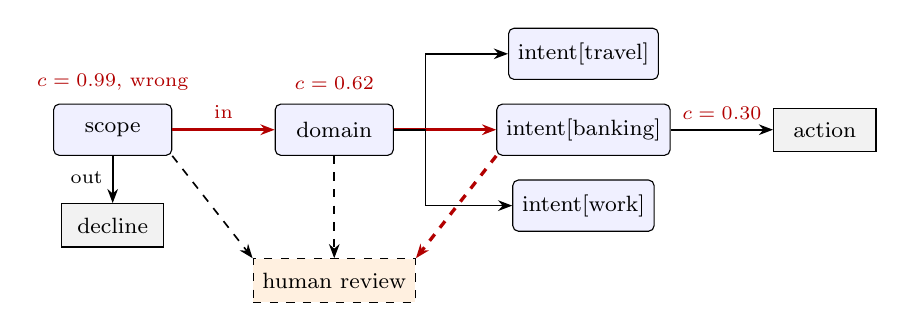
\begin{tikzpicture}[font=\footnotesize, node distance=6mm and 13mm,
  dec/.style={draw, rounded corners=2pt, minimum height=6.5mm, minimum width=15mm, fill=blue!6},
  snk/.style={draw, minimum height=5.5mm, minimum width=13mm, fill=black!5},
  hum/.style={draw, dashed, minimum height=5.5mm, minimum width=20mm, fill=orange!12},
  arr/.style={-{Stealth[length=1.8mm]}, semithick},
  run/.style={-{Stealth[length=1.8mm]}, very thick, red!70!black}]
\node[dec] (scope) {scope};
\node[dec, right=of scope] (domain) {domain};
\node[dec, right=of domain] (intent) {intent[banking]};
\node[dec, above=3mm of intent] (i1) {intent[travel]};
\node[dec, below=3mm of intent] (i2) {intent[work]};
\node[snk, right=of intent] (act) {action};
\node[snk, below=of scope] (oos) {decline};
\node[hum, below=13mm of domain] (human) {human review};
\draw[arr] (scope) -- node[left, pos=.45]{\scriptsize out} (oos);
\draw[run] (scope) -- node[above]{\scriptsize in} (domain);
\draw[arr] (domain.east) -- ++(4mm,0) |- (i1.west);
\draw[run] (domain) -- (intent);
\draw[arr] (domain.east) -- ++(4mm,0) |- (i2.west);
\draw[arr] (intent) -- node[above, red!70!black] {\scriptsize $c=0.30$} (act);
\draw[arr, dashed] (scope.south east) -- (human.north west);
\draw[arr, dashed] (domain) -- (human);
\draw[run, dashed] (intent.south west) -- (human.north east);
\node[above=0.5mm of scope, red!70!black] {\scriptsize $c=0.99$, wrong};
\node[above=0.5mm of domain, red!70!black] {\scriptsize $c=0.62$};
\end{tikzpicture}
\caption{A decision workflow and a rescued error. An out-of-scope request is confidently
passed by \texttt{scope} (the first error), reaches nodes that were not built for it, and is
escalated by an unsure \texttt{intent} node. Charging the run to its first error counts it as
an error at every threshold below $0.99$; charging it to the least confident node counts it
only when $\tau_{\text{intent}}\le0.30$, which is when it actually completes.}
\label{fig:workflow}
\end{figure}

We also state plainly what the results do not show. Uniform certificates are not free: at a
fixed target, end-to-end Pareto testing~\citep{laufer2022pareto} escalates less than any
certificate that remains valid under retuning. A certificate cannot repair a model: the
token probabilities of a zero-shot language model are close to uninformative at one of our
nodes, and there the honest outcome is a refusal. And the guarantees are for exchangeable
traffic (\S\ref{sec:limits}).

\section{Setting}\label{sec:setting}

\paragraph{Workflows.} A workflow has a finite set $V$ of decision nodes. Node $v$ receives a
state $s$ and returns a choice $\hat y_v(s)$ from a finite set $C_v$ together with a confidence
$c_v(s)\in[0,1]$. Each choice leads either to another decision node or to a sink; the successor
relation is acyclic. Everything between two decisions (formatting, retrieval, deterministic
transforms) is folded into the state passed along the edge, which is a function of the
previous state and the choice taken.

\paragraph{Runs.} An input $x\sim P$ enters at the root. Its \emph{free run} $\pi(x) =
(v_1,\dots,v_m)$ is the sequence of nodes visited when every node commits to its top choice,
with confidences $c_1(x),\dots,c_m(x)$. The free run does not involve the thresholds. Given
thresholds $\tau\in([0,1]\cup\{\infty\})^V$, the workflow follows the free run and escalates at
the first node whose confidence is below its threshold; $\tau_v=\infty$ means $v$ never commits.
The run \emph{completes} when no node escalates:
\[
\Comp(\tau)=\bigl\{x:\ c_j(x)\ge\tau_{v_j}\ \text{for all } j\le m\bigr\}.
\]

\paragraph{Errors.} Ground truth assigns to each input its \emph{oracle route} $\pi^*(x)$, the
route obtained when every decision is correct. Let $D=\{x:\pi(x)\ne\pi^*(x)\}$ be the inputs
whose free run deviates. An escalated run is resolved by a human and is not an error. The
\emph{risk} and the \emph{review rate} are
\[
R(\tau)=\Prob\bigl(D\cap\Comp(\tau)\bigr),\qquad H(\tau)=1-\Prob\bigl(\Comp(\tau)\bigr).
\]
The goal is to choose $\tau$ from $n$ labelled calibration inputs so that $R(\tau)\le\eps$ with
probability at least $1-\delta$ over the calibration sample, and $H(\tau)$ is small.

\paragraph{Assumptions.} (A1) Calibration and deployment inputs are i.i.d.\ from $P$. (A2) The
state a node receives depends only on the input and the choices taken before it, so the free
run is well defined and deterministic given $x$. (A3) Labels identify the oracle route. We
present the case where each run is a path. If a choice feeds several decision nodes, $\pi(x)$
is the set of visited nodes and every statement below holds with ``on the route'' read as ``in
the visited set''.

\section{Separable certificates}\label{sec:sep}

\subsection{The charging lemma}

\begin{definition}
A \emph{charging rule} is a map $u:D\to V$ with $u(x)\in\pi(x)$: it assigns every deviating
free run to one node on its route. It may depend on the models and the labels but not on
$\tau$. We write $c_u(x)$ for the confidence of $u(x)$ on the free run of $x$.
\end{definition}

\begin{lemma}[Charging]\label{lem:charging}
For every charging rule $u$ and every $\tau$,
\[
R(\tau)\ \le\ B_u(\tau):=\sum_{v\in V}\rho^u_v(\tau_v),\qquad
\rho^u_v(t)=\Prob\bigl(x\in D,\ u(x)=v,\ c_u(x)\ge t\bigr).
\]
Each $\rho^u_v$ is non-increasing and depends on $\tau$ only through $\tau_v$. The gap is
$B_u(\tau)-R(\tau)=\Prob\bigl(x\in D,\ c_u(x)\ge\tau_{u(x)},\ x\notin\Comp(\tau)\bigr)$.
\end{lemma}
\begin{proof}
If $x\in D\cap\Comp(\tau)$ then every node on $\pi(x)$ has confidence at least its threshold,
in particular $u(x)$. Hence $D\cap\Comp(\tau)\subseteq\{x\in D: c_u(x)\ge\tau_{u(x)}\}$, and the
right-hand side is the disjoint union over $v$ of the events defining $\rho^u_v(\tau_v)$. The
gap is the probability of the set difference.
\end{proof}

The lemma is elementary, and that is its value: the dependence between nodes, which is what
makes multi-stage calibration hard, is absorbed into the choice of $u$, after which each node
contributes a curve of its own threshold. The gap consists of deviating runs whose charged
node commits while another node on the route escalates. We call these runs \emph{rescued}.

\subsection{Three rules}\label{sec:rules}

\paragraph{First error (FE).} $u(x)$ is the first node of the free run whose choice is wrong.
This is the rule one arrives at by extending additive stage-wise decompositions for
cascades~\citep{sun2026compcrc} to routing: every error is attributed to the stage that caused
it. It needs only free-run logs. Its weakness is that it ignores everything after the first
error. In a routing workflow the first error sends the input to nodes that were never meant to
see it, and those nodes are often unsure; FE charges the run as if they had all committed.

\paragraph{Teacher forced (TF).} Charge \emph{every} node that is wrong on the state it
receives along the oracle route, whether or not the free run reaches it:
$\rho^{\mathrm{TF}}_v(t)=\Prob(v\in\pi^*(x),\ \hat y_v\ne y_v,\ c_v\ge t)$ evaluated on
oracle-route states. Since the first wrong node of a deviating run is wrong on its oracle-route
state, $\rho^{\mathrm{FE}}_v\le\rho^{\mathrm{TF}}_v$ and the bound of Lemma~\ref{lem:charging}
still holds, now as a union bound. TF is the most modular rule: $\rho^{\mathrm{TF}}_v$ depends
on no other node's model, and factors as $\Prob(v\in\pi^*)$ times a selective error of $v$ on
its own domain, which a component owner could certify in isolation. It is also the loosest.

\paragraph{Least confident (LC).} $u(x)$ is the node of the free run with the smallest
confidence, or more generally the smallest margin $c_j(x)-a_{v_j}$ for a fixed anchor
$a\in\mathbb{R}^V$. Ties go to the first wrong node if it is among the minimisers and to the
earliest node otherwise; they matter when confidences saturate (\S\ref{sec:exp-llm}). The rule looks at the whole route, so it sees
rescue.

\begin{proposition}[Exactness]\label{prop:exact}
For the LC rule with anchor $a$, $B_u(a+s\mathbf{1})=R(a+s\mathbf{1})$ for every $s$. In
particular the unanchored rule is exact whenever all thresholds are equal.
\end{proposition}
\begin{proof}
With $\tau=a+s\mathbf 1$, a run completes iff $\min_j\,(c_j-a_{v_j})\ge s$, i.e.\ iff the node
attaining the minimum has $c_u\ge a_{u}+s=\tau_{u}$. So $\{x\in D:c_u\ge\tau_u\}=D\cap\Comp(\tau)$.
\end{proof}

An anchor can be learned on a tuning split (for instance, thresholds proposed by an
end-to-end heuristic), which makes the bound exact along a ray through a good configuration
while it remains valid everywhere.

\subsection{A uniform finite-sample certificate}

Partition $V$ into $M$ \emph{modules}; nodes of a module share one threshold. Modules control
granularity: one per node, one per level of the workflow, or a single one. Fix a finite grid
$\mathcal G\subset[0,1]\cup\{\infty\}$ of $G$ thresholds containing $\infty$. An assignment
$g\in\mathcal G^M$ induces thresholds $\tau_g$. Given calibration inputs $x_1,\dots,x_n$, let
\[
k_m(t)=\#\{i:\ x_i\in D,\ u(x_i)\in m,\ c_u(x_i)\ge t\},\qquad k(g)=\sum_{m=1}^M k_m(g_m).
\]
Let $\CP(k,n,\alpha)$ denote the one-sided Clopper--Pearson upper confidence bound at level
$1-\alpha$ for a binomial proportion with $k$ successes in $n$ trials~\citep{clopper1934}.

\begin{theorem}[Certificate]\label{thm:cert}
Let $u$ be a charging rule fixed independently of the calibration sample, and set
$U(g)=\CP\bigl(k(g),n,\delta/G^M\bigr)$ for $g\ne(\infty,\dots,\infty)$ and $U(\infty,\dots,\infty)=0$.
Under \textup{(A1)--(A3)}, with probability at least $1-\delta$,
\[
R(\tau_g)\le U(g)\qquad\text{simultaneously for all } g\in\mathcal G^M.
\]
\end{theorem}
\begin{proof}
Fix $g$. Each calibration input contributes to $k(g)$ at most once, because it is charged to
one node, and does so with probability $B_u(\tau_g)$. So $k(g)\sim\mathrm{Bin}(n,B_u(\tau_g))$
and $\Prob(B_u(\tau_g)>U(g))\le\delta/G^M$. A union bound over the fewer than $G^M$ assignments
other than all-$\infty$ and Lemma~\ref{lem:charging} give the claim; a workflow that never
commits has risk exactly zero.
\end{proof}

\begin{corollary}[Post hoc selection]\label{cor:posthoc}
On the event of Theorem~\ref{thm:cert}, every assignment $\hat g$ with $U(\hat g)\le\eps$
satisfies $R(\tau_{\hat g})\le\eps$, however $\hat g$ and $\eps$ were chosen---including after
inspecting the calibration data and the certificate, and for several targets at once.
\end{corollary}

Three remarks. \emph{(i) Sufficient statistics.} The certificate is the $M\times G$ integer
table $k_m(t)$ and $n$; no raw inputs or labels need to be retained. \emph{(ii) One bound, not
$M$.} Because each run is charged once, the per-node terms pool into a single binomial count.
Bounding the $M$ curves separately and adding the bounds is also valid, and is what TF
requires, but pays $M$ confidence margins instead of one. \emph{(iii) The price of
uniformity.} With no observed errors the bound is about $(M\ln G+\ln\frac1\delta)/n$. Tying
thresholds lowers $M$. Some dependence on $M$ is inherent in bounds that hold for all
thresholds at once, as the family of completion events has VC dimension $M$; we do not claim
the constant is optimal.

\subsection{Choosing thresholds}

Let $k_{\max}(\eps)$ be the largest count with $\CP(k,n,\delta/G^M)\le\eps$. Selecting thresholds
means choosing one grid value per module with total charged count at most $k_{\max}$. As
objective we use the separable surrogate $\sum_m h_m(g_m)$, where $h_m(t)$ is the fraction of
calibration runs that visit a node of module $m$ with confidence below $t$; it upper-bounds the
review rate by a union bound. The result is a multiple-choice knapsack problem with integer
weights~\citep{kellerer2004}, solved exactly by dynamic programming in $O(MG\,k_{\max})$ time.
Since the certificate is uniform, the solution may then be refined by any local search on the
empirical review rate without affecting validity; we use coordinate descent.

\section{Edits}\label{sec:edits}

\subsection{Locality}

Let $W'$ be obtained from a workflow $W$ by an \emph{edit} of a set $E\subseteq V$: the models
of the nodes in $E$, their choice sets, and anything reachable only through them may change
(including new nodes); every other node and the labels of the unedited decisions are unchanged.
Let $T_E=\{x:\pi_W(x)\cap E\ne\emptyset\}$ be the inputs whose free run meets the edit.

\begin{proposition}[Locality]\label{prop:local}
\textup{(i)} The free run of $x$ in $W'$ meets $E$ if and only if $x\in T_E$.
\textup{(ii)} For $x\notin T_E$ the free run, its confidences, and whether it deviates are the
same in $W$ and $W'$. Consequently, for every $\tau$,
\[
R_{W'}(\tau)=\Prob\bigl(D_W\cap\Comp_W(\tau)\cap T_E^{\,c}\bigr)
+\Prob(T_E)\,\Prob\bigl(D_{W'}\cap\Comp_{W'}(\tau)\mid T_E\bigr).
\]
\end{proposition}
\begin{proof}
The part of a free run before its first node in $E$ consists of unedited nodes receiving the
same states, so it is identical in $W$ and $W'$; this gives (i), and for $x\notin T_E$ the
whole run is identical. Such a run deviates iff it differs from the oracle route. If the
oracle route avoids $E$ it is unchanged by the edit. If it meets $E$ in either workflow it
meets $E$ in both, because its prefix up to $E$ is determined by unedited labels, and then the
run, which avoids $E$, deviates in both. The displayed identity is the law of total
probability.
\end{proof}

\subsection{Route-indexed certificates}

Proposition~\ref{prop:local} says that the old calibration sample remains evidence about the
first term, exactly, for any charging rule. To use it, the certificate must be able to separate
the runs that meet $E$ from those that do not, for an $E$ unknown when it is issued. Storing
the count curves \emph{per free route} achieves this: the table becomes
$k_{r,m}(t)$ for each distinct route $r$, and the curves for the traffic avoiding $E$ are
obtained by summing over the routes that do not contain a node of $E$.

\begin{theorem}[Edit-local recertification]\label{thm:recert}
Let $u$ be a charging rule for $W$ and $u'$ one for $W'$, and let $E$ be chosen independently
of the samples. Let $k^{\circ}(g)$ be the charged count of the old sample ($n$ runs of $W$)
restricted to runs outside $T_E$, let $r$ be the number of old runs in $T_E$, and let $k'(g)$
be the charged count of $m$ fresh runs of $W'$ drawn i.i.d.\ from $P(\cdot\mid T_E)$. Then with
probability at least $1-\delta_0-\delta_1-\delta_2$, simultaneously for all $g\in\mathcal G^M$,
\[
R_{W'}(\tau_g)\ \le\ \CP\bigl(k^{\circ}(g),n,\delta_0/G^{M}\bigr)
+\CP(r,n,\delta_1)\cdot\CP\bigl(k'(g),m,\delta_2/G^{M_E}\bigr),
\]
where $M_E$ is the number of modules with a node on some route through $E$.
\end{theorem}
\begin{proof}
Apply Lemma~\ref{lem:charging} to each term of Proposition~\ref{prop:local}. For fixed $g$,
$k^\circ(g)$ is binomial with $n$ trials and success probability at least the first term;
$r$ is binomial with success probability $\Prob(T_E)$ and needs no labels; and $k'(g)$ is
binomial with $m$ trials and success probability at least the conditional risk. The fresh
term depends on $g$ only through the $M_E$ modules that occur on routes through $E$. A union
bound over the grid and over the three events concludes.
\end{proof}

The fresh sample is drawn from the traffic that reaches the edited node, which is what an
operator can collect cheaply after a change: log the runs through the new node and label
those. Its bound is multiplied by the traffic share, so a node that handles 9\% of the traffic
needs roughly one eleventh of the labels for the same contribution to the bound. The theorem
iterates: after a second edit the remaining routes of every earlier part are kept, and the
share of the new edit is bounded from the original sample.

\subsection{Node-level footprints}\label{sec:footprint}

Without route indexing, one can still ask which per-node curves an edit of a single node $w$
invalidates. The answer depends on the charging rule and is the reverse of its tightness.

\begin{proposition}[Footprints]\label{prop:footprint}
After editing the model of $w$: under \textup{TF} only the curve of $w$ can change; under
\textup{FE} only the curves of $w$ and its descendants; under \textup{LC} the curve of any node
that shares a route with $w$.
\end{proposition}
\begin{proof}
The TF event of $v$ involves only $v$'s output on oracle-route states. The FE event of $v$ is
``$v$ is on the oracle route, all nodes before it on that route are correct, $v$ is wrong and
commits'', which involves $v$ and its ancestors, so it can change only if $w$ is $v$ or an
ancestor of $v$. The LC event of $v$ depends on the confidences along the run.
\end{proof}

So the rules trade tightness for stability at node granularity. Route indexing sidesteps the
trade: locality is a property of the traffic, not of the rule, and holds for the tight LC rule
(Table~\ref{tab:footprints} verifies both statements on data).

\subsection{A static check}\label{sec:impl}

We implemented the certificate in \anp, a runtime that executes workflows given as JSON graphs
of typed nodes. A \texttt{decision} node carries a question, a closed choice set, a threshold
and an \texttt{uncertain} port; the runtime routes each input to the port of the winning choice
or to \texttt{uncertain}. The command \texttt{anp certify} turns labelled free-run traces into
a route-indexed certificate, solves the knapsack for a target $\eps$ and writes the thresholds
back into the graph. Each decision node is fingerprinted by its configuration without the
thresholds, together with the decision nodes its ports lead to. \texttt{anp verify -{}-risk}
then fails a graph (i) whose thresholds, rounded down to the grid, have a certified bound above
$\eps$, or (ii) in which a decision node's fingerprint differs from the certificate's, naming
the nodes whose traffic must be relabelled; \texttt{anp certify -{}-fresh} performs the repair of
Theorem~\ref{thm:recert}. Thresholds can be raised freely, and edits to non-decision nodes that
keep the routing leave the certificate valid. The implementation is independent of the Python
code used for the experiments and is tested against it on real traces.

\section{Experiments}\label{sec:exp}

\paragraph{Setup.} We build two workflows from public intent-classification data
(details in Appendix~\ref{app:details}). \textbf{CLINC150}~\citep{larson2019clinc}: a
\texttt{scope} node separates in-scope from out-of-scope requests, a \texttt{domain} node
picks one of 10 product areas, and one \texttt{intent} node per area picks among its 15
intents: 12 decisions on a tree of depth 3 (Figure~\ref{fig:workflow}).
\textbf{MASSIVE}~\citep{fitzgerald2022massive} in four languages: a \texttt{language} node, a
\texttt{scenario} node per language (18 scenarios), and an \texttt{intent} node per scenario
that is shared by all languages: 21 decisions on a DAG with joins. Every node is a logistic
regression on frozen sentence embeddings~\citep{reimers2019sbert}, trained on the training
split; its confidence is the top class probability. Without abstention the workflows err on
\FreeErrClinc\% and \FreeErrMassive\% of inputs.

To measure validity without test-set noise we treat the pooled held-out data (8{,}600 and
20{,}028 inputs) as the population: a calibration set is $n$ i.i.d.\ draws from it, and each
selected threshold vector is scored by its exact risk and review rate on the population. We
report means over repeated draws and the \emph{violation rate}, the fraction of draws whose
population risk exceeds $\eps$; a method with a $(1-\delta)$ guarantee must keep it below
$\delta=0.1$.

\paragraph{Methods.} Without guarantee: a fixed threshold of 0.7; \emph{per-node selective
risk}, which tunes each node separately so that its own error rate among committed inputs is
certified below $\eps$; and a \emph{plug-in} version of our certificate without confidence
bounds. End to end, valid for one pre-specified target: a single \emph{shared threshold}
calibrated by fixed-sequence testing on the exact risk~\citep{angelopoulos2021ltt}, the
selective-risk counterpart of joint-score calibration~\citep{ren2023knowno,kotte2026pasc}; and
\emph{Pareto testing}~\citep{laufer2022pareto} over per-node thresholds, with half of the
data proposing candidates and half testing them. Uniform over the grid: an \emph{end-to-end
uniform} bound on the exact error count with the same union as Theorem~\ref{thm:cert}; and
our certificates with TF, FE and LC charging, with modules per node, per level, or shared.

\subsection{Validity and efficiency}\label{sec:exp-main}

\begin{table}[t]
\centering\footnotesize
\setlength{\tabcolsep}{3.5pt}
\begin{tabular}{llrrrrrrrrr}
\toprule
 & & \multicolumn{3}{c}{$\varepsilon=2\%$} & \multicolumn{3}{c}{$\varepsilon=5\%$} & \multicolumn{3}{c}{$\varepsilon=10\%$} \\
\cmidrule(lr){3-5}\cmidrule(lr){6-8}\cmidrule(lr){9-11}
Method & Guarantee & viol. & risk & review & viol. & risk & review & viol. & risk & review \\
\midrule
Fixed threshold 0.7 & none & 100 & 4.6 & 22.5 & 0 & 4.6 & 22.5 & 0 & 4.6 & 22.5 \\
Per-node selective risk & none & 0 & 0.0 & 100.0 & 0 & 1.7 & 76.6 & 100 & 12.3 & 10.1 \\
Plug-in (no confidence bound) & none & 68 & 2.1 & 37.0 & 64 & 5.1 & 20.4 & 54 & 10.0 & 8.3 \\
\midrule
Shared threshold, end-to-end LTT & fixed & 1 & 1.4 & 53.1 & 0 & 4.1 & 25.2 & 0 & 8.6 & 11.6 \\
End-to-end Pareto testing & fixed & 2 & 1.4 & 49.9 & 3 & 4.1 & 25.0 & 3 & 8.6 & 11.6 \\
End-to-end, uniform over grid & uniform & 0 & 0.6 & 67.7 & 0 & 2.4 & 36.4 & 0 & 6.2 & 17.8 \\
\midrule
Teacher-forced, per node & uniform & 0 & 0.0 & 100.0 & 0 & 0.2 & 87.2 & 0 & 2.5 & 41.1 \\
First-error, per node & uniform & 0 & 0.0 & 100.0 & 0 & 0.7 & 73.9 & 0 & 3.9 & 36.6 \\
First-error, per level & uniform & 0 & 0.0 & 99.4 & 0 & 0.9 & 58.9 & 0 & 5.8 & 30.1 \\
\midrule
Least-confident, per node & uniform & 0 & 0.5 & 64.7 & 0 & 2.4 & 34.3 & 0 & 6.2 & 17.4 \\
Least-confident, per level & uniform & 0 & 1.0 & 50.3 & 0 & 3.4 & 27.8 & 0 & 7.8 & 13.6 \\
Least-confident, shared & uniform & 0 & 1.1 & 61.4 & 0 & 3.7 & 27.1 & 0 & 8.1 & 12.8 \\
Anchored, per level & uniform & 0 & 0.7 & 61.6 & 0 & 3.1 & 29.7 & 0 & 7.3 & 14.7 \\
\bottomrule
\end{tabular}

\caption{CLINC150, $n=4{,}000$, $\delta=0.1$, \Trials\ calibration draws. \emph{viol.}:
percentage of draws with population risk above $\eps$ (bold: above $\delta$ for a method
that claims a guarantee); \emph{risk}, \emph{review}: mean population risk and human review
rate in percent. ``fixed'': valid for the single target it was run for; ``uniform'': valid
for all thresholds on the grid at once.}\label{tab:main}
\end{table}

Table~\ref{tab:main} gives the results for CLINC150 and Table~\ref{tab:main-massive} in the
appendix for MASSIVE.

\paragraph{Uncertified practice fails where it matters.} Per-node selective calibration
controls each node's own error rate and ignores that errors accumulate along a route: at
$\eps=10\%$ it exceeds the target in \ViolCPerNodeTen\% of draws on CLINC150 and
\ViolMPerNodeTen\% on MASSIVE. The plug-in certificate, which uses frequencies in place of
confidence bounds, violates in \ViolCPlugFive\% and \ViolMPlugFive\% of draws at $\eps=5\%$.
Every method with a guarantee stays within $\delta$: the largest violation rate among them, over both workflows and
all targets, is \MaxViolCertified\%.

\paragraph{The rescue effect.} FE and TF certificates are valid but nearly useless on
CLINC150: at $\eps=5\%$ they escalate \RevCFEnodeFive\% and \RevCTFnodeFive\% of inputs, against
\RevCLCnodeFive\% for LC with the same per-node modules and the same union bound. The reason is
visible in the population. At the thresholds chosen by the shared end-to-end method for
$\eps=5\%$, the mass of deviating runs whose first wrong node commits is \FdMassC\%, while the
actual risk is \RiskCSharedFive\%: \RescuedShareC\% of the first-error mass is escalated
further along the route. The \texttt{scope} node passes out-of-scope requests with high
confidence, and the \texttt{domain} and \texttt{intent} nodes, facing inputs unlike anything
they were trained on, hesitate. On MASSIVE, where errors are spread over more nodes, the
first-error mass still overstates the risk by a factor of \FdRatioM\ (\RescuedShareM\%
rescued), and FE needs \RevMFEnodeFive\% review where LC needs \RevMLCnodeFive\%. Additive
attribution to the causing stage, which is exact for a cascade of interchangeable solvers,
therefore misjudges routing workflows.

\paragraph{The price of uniformity and of granularity.} Among the certified methods, Pareto
testing escalates least at a fixed target (\RevCParetoFive\% on CLINC150 and
\RevMParetoFive\% on MASSIVE at $\eps=5\%$), as it tests a short pre-ordered list of
configurations and pays no union over the grid. Certificates that stay valid under retuning
pay for it: LC per level needs \RevCLClevelFive\% and \RevMLClevelFive\%, LC per node
\RevCLCnodeFive\% and \RevMLCnodeFive\%. The separable bound is not the bottleneck: the
end-to-end uniform bound, which uses exact error counts and the same union, needs
\RevCUnifFive\% and \RevMUnifFive\%, no less than LC per node, because its feasible set can
only be searched heuristically whereas the separable problem is solved exactly. With a single
shared module the LC certificate uses exactly the end-to-end error counts
(Proposition~\ref{prop:exact}); its remaining distance to the shared-threshold baseline
(\RevCLCsharedFive\% against \RevCSharedFive\%) is the union over the grid. How much there is
to gain from per-node thresholds depends on the workflow: with thresholds optimised directly
on the population, per-node thresholds reach $\eps=5\%$ at \OracleNodeCFive\% review against
\OracleSharedCFive\% for the best shared threshold on CLINC150, and \OracleNodeMFive\% against
\OracleSharedMFive\% on MASSIVE. Tying thresholds by level is a good default: it keeps most of
the control and pays the union for three modules only.

\subsection{Calibration size and number of decisions}

\begin{figure}[t]
\centering
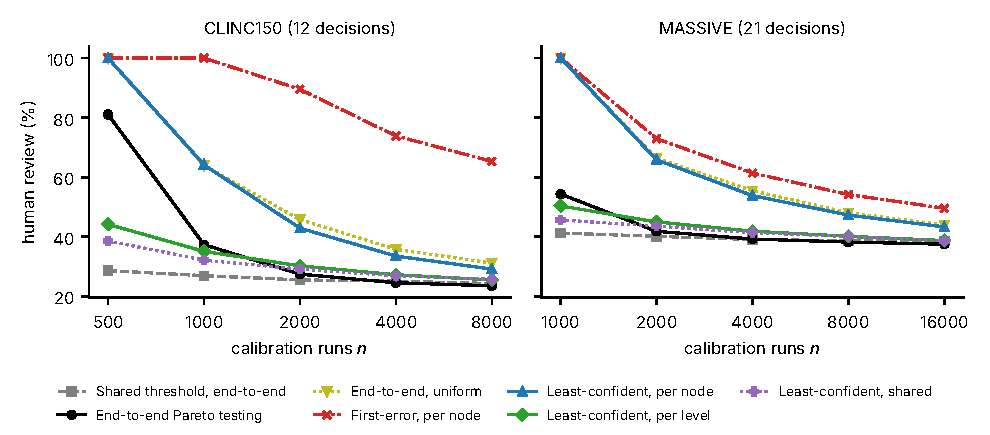
\includegraphics[width=\linewidth]{figures/nsweep.pdf}
\caption{Human review needed to certify $\eps=5\%$ as a function of the calibration size
(\NsweepTrials\ draws per point, $\delta=0.1$).}\label{fig:nsweep}
\end{figure}

\begin{figure}[t]
\centering
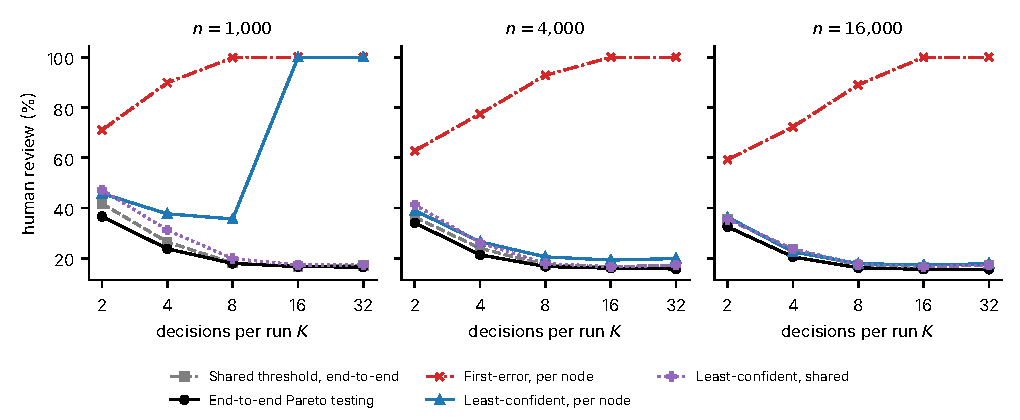
\includegraphics[width=\linewidth]{figures/synth.pdf}
\caption{Synthetic chains of $K$ decisions with 20\% erroneous runs before abstention:
review needed to certify $\eps=5\%$ (\SynthTrials\ draws per point). The per-node certificate
pays a union over $K$ thresholds; a shared module does not.}\label{fig:synth}
\end{figure}

Figure~\ref{fig:nsweep} varies $n$. The gap between uniform and fixed-target methods is a
statistical margin and closes as $n$ grows; with few calibration runs, fine-grained uniform
certificates cannot certify at all, and the shared and per-level variants degrade most
gracefully. Figure~\ref{fig:synth} isolates the dependence on the number of decisions with
synthetic chains in which every run visits all $K$ nodes, node errors are correlated through
a shared difficulty, and confidences are overconfident. The per-node certificate needs
\SynthTwoSmallLCnode\% review for $K=2$ and \SynthThirtyTwoSmallLCnode\% for $K=32$ at
$n=1{,}000$, and \SynthTwoLargeLCnode\% and \SynthThirtyTwoLargeLCnode\% at $n=16{,}000$,
consistent with a margin of order $K\ln G/n$; the shared module is insensitive to $K$. FE
charging is loose throughout because the chains have rescue by construction.

\subsection{Post hoc retuning}

\begin{figure}[t]
\centering
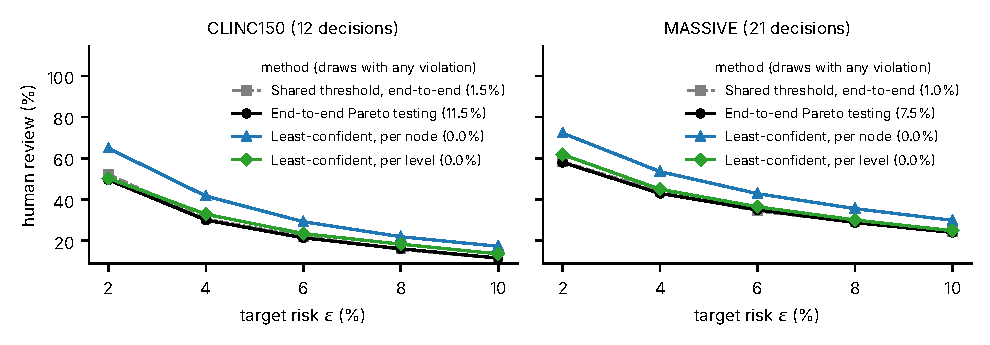
\includegraphics[width=\linewidth]{figures/posthoc.pdf}
\caption{One calibration set, five targets. The LC certificates are issued once and
re-optimised for each $\eps$; the end-to-end procedures are re-run for each $\eps$ on the same
data. In parentheses: percentage of calibration draws in which at least one of the five
selected configurations violates its target (\PosthocTrials\ draws).}\label{fig:posthoc}
\end{figure}

Operators rarely keep one target. Figure~\ref{fig:posthoc} issues a certificate once and then
selects thresholds for five targets from 2\% to 10\%. For the LC certificates this is covered
by Corollary~\ref{cor:posthoc}: in \AnyViolCLClevel\% (CLINC150) and \AnyViolMLClevel\%
(MASSIVE) of draws at least one of the five configurations violates its target. Re-running
an end-to-end procedure for each target on the same data is not covered by its guarantee.
In our experiments the simultaneous violation rates of the re-run procedures are
\AnyViolCPareto\% and \AnyViolMPareto\% for Pareto testing and \AnyViolCShared\% and
\AnyViolMShared\% for the shared threshold; the selected configurations are strongly
dependent across targets, so the inflation over the per-target level is modest here, but
nothing bounds it in general.

\subsection{Edits}\label{sec:exp-edits}

\begin{figure}[t]
\centering
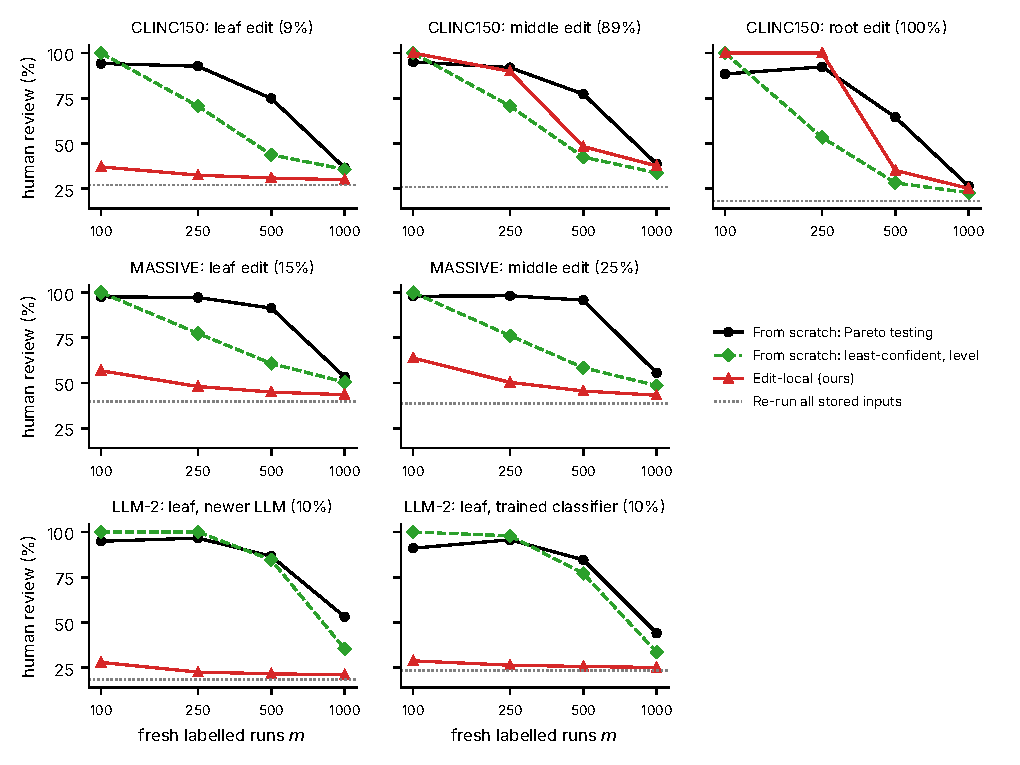
\includegraphics[width=\linewidth]{figures/edits.pdf}
\caption{Review needed to certify $\eps=5\%$ after replacing the model of one node, as a
function of the number $m$ of fresh labelled runs (\EditTrials\ draws per point). \emph{From
scratch} labels $m$ runs of all traffic and recalibrates with them alone. \emph{Edit-local}
(Theorem~\ref{thm:recert}) keeps the old certificate for the routes that avoid the node and
labels $m$ runs of the traffic through it. The dotted line recalibrates on all stored inputs
re-run through the edited workflow, which assumes they were kept.}\label{fig:edits}
\end{figure}

We replace the model of one node by a model from a different family and ask how many fresh
labels are needed to certify the edited workflow at $\eps=5\%$ (Figure~\ref{fig:edits}). The
old certificate was issued from $n$ runs of the unedited workflow. We first confirmed
Proposition~\ref{prop:local} on the populations: for each edit, the runs that avoid the
edited node have identical routes, confidences and deviation status before and after.

For a leaf (\EditShareCLeaf\% of the traffic on CLINC150, \EditShareMLeaf\% on MASSIVE) the
edit-local certificate needs \EditCLeafLocalHundred\% and \EditMLeafLocalHundred\% review with
$m=100$ fresh labels. Recalibrating from scratch with 100 labels certifies nothing
(\EditCLeafScratchHundred\% and \EditMLeafScratchHundred\% review with Pareto testing), and
with $m=1{,}000$ it reaches \EditCLeafScratchThousand\% and \EditMLeafScratchThousand\%, where
the edit-local certificate is at \EditCLeafLocalThousand\% and \EditMLeafLocalThousand\%. For a
middle node the picture depends on its traffic share: a \texttt{scenario} node of MASSIVE
(\EditShareMMiddle\% of the traffic) is repaired locally with 100 labels at
\EditMMiddleLocalHundred\% review, while the \texttt{domain} node of CLINC150 carries
\EditShareCMiddle\% of the traffic, leaves little to reuse, and gains nothing from
locality. Editing the root touches every run, and the edit-local procedure then reduces to
recalibration from scratch with a smaller share of $\delta$. Across all edits and sample sizes
the largest violation rate of the edit-local certificates is \EditMaxViolLocal\%.

If all calibration inputs and labels were retained, re-running them through the edited
workflow and recalibrating is at least as good (dotted line); that option requires storing
raw inputs, and each such recalibration is a new certificate for a single configuration. The
edit-local certificate needs only the stored counts.


\section{Related work}\label{sec:related}

\paragraph{Risk control and selective prediction.} Abstaining to bound error goes back to
\citet{chow1970}; \citet{geifman2017selective} gave finite-sample guarantees for a single
selective classifier. Conformal prediction~\citep{vovk2005} and its risk-controlling
extensions~\citep{bates2021rcps,angelopoulos2021ltt,angelopoulos2022crc} certify
hyperparameters of arbitrary predictors; Pareto testing~\citep{laufer2022pareto} makes
multi-dimensional configurations tractable by ordering candidates on a split and testing them
in sequence. We use these tools as baselines and building blocks. They certify a
pre-specified system and a pre-ordered set of candidates; our certificate is uniform over a
product grid and is designed to be repaired.

\paragraph{Guarantees for multi-stage LLM systems.} For language models, abstention with
guarantees has been studied for single calls~\citep{yadkori2024abstention} and for judges that
escalate to humans~\citep{jung2024trust}. Multi-stage guarantees have mostly been obtained in
two ways. One calibrates a single scalar over whole trajectories: KnowNo~\citep{ren2023knowno}
for multi-step robot planning and PASC~\citep{kotte2026pasc} for NLP pipelines; this is tight
for one shared threshold, which corresponds to our LC rule with a single module, and must be
redone when the pipeline changes. The other splits an error budget across components by a
union bound, as in TRAQ for retrieval and generation~\citep{li2023traq} and in model
cascades~\citep{chen2023frugalgpt,dou2026cascade,xu2025selective}. Closest to ours, the
concurrent CompCRC~\citep{sun2026compcrc} decomposes the accepted-error risk of a linear
cascade into additive stage contributions and certifies each stage against a local budget. Its
stage losses include a reach indicator that depends on upstream thresholds, its guarantee is in
expectation for thresholds fixed before certification, and it explicitly excludes post hoc
budget selection. Our charged terms depend on one threshold each, hold uniformly, and apply to
routing DAGs in which stages solve different sub-problems; we also show that the first-error
attribution underlying additive decompositions is loose under routing. Hierarchical selective
classification~\citep{goren2024hierarchical} retreats to coarser labels of a single model
rather than escalating a multi-model program. \citet{chatrath2026ready} argue for qualifying
whole workflows on held-out data; we give that qualification a form that persists across
edits.

\paragraph{Languages for model-driven programs.} Declarative
frameworks~\citep{khattab2023dspy} and typed calculi and languages for agent
composition~\citep{liu2026lambda,kizito2026turn} treat model calls as program constructs, the
latter exposing a confidence value to the program. None attaches a statistical guarantee to
the program or tracks its validity under edits; our static check is a step in that direction.

\section{Limitations}\label{sec:limits}

\emph{Exchangeability.} All guarantees assume calibration and deployment traffic are i.i.d.
Under drift the certificate is evidence about the past. Edit locality does not help here; it
concerns changes to the program, not to the world.
\emph{Labels.} Calibration needs the oracle route of each input. In our datasets one label
determines the route; in general each decision may need its own annotator.
\emph{Model class.} The method is agnostic to how confidences are produced. Most of our
experiments use classifiers on frozen sentence embeddings. The language-model experiment uses
one provider, two models, zero-shot prompts and a single task; its token probabilities
saturate, which leaves thresholds little to work with, and we did not study verbalised or
sampled confidences, few-shot prompting at scale, or fine-tuned models.
\emph{Structure.} We assume acyclic routing, deterministic states and an escalation that fully
resolves the run. Loops, stochastic nodes and partial human corrections are out of scope.
\emph{Adaptive edits.} Theorem~\ref{thm:recert} requires the edited set to be chosen
independently of the calibration sample; choosing which node to replace by inspecting the
certificate calls for a union over the candidate edits. Each repair also spends additional
failure probability, so a long edit history eventually warrants a fresh certificate.
\emph{Efficiency.} Uniform validity costs review at a fixed target relative to end-to-end
testing (\S\ref{sec:exp-main}), and the grid and the union bound are simple rather than
optimal.

\section{Conclusion}

Calibration guarantees for multi-step systems are usually stated for a frozen system, while
the systems themselves are edited continuously. We showed that two structural facts make
guarantees more durable: errors can be charged to single nodes so that the risk bound
separates across thresholds, and an edit is confined to the traffic that passes through it.
Together they give certificates that remain valid when thresholds are retuned and that can be
repaired locally when a node changes, at a statistical price we quantified. The negative
results are as useful as the positive ones: blaming the first error, the intuitive way to
compose stage-wise guarantees, can misjudge routing workflows, because what goes wrong
upstream is often caught downstream.

\paragraph{Reproducibility.} Code for the experiments, the exported traces of one workflow,
and the runtime implementation are available in the project repository under
\texttt{paper/} and \texttt{examples/certify/}. A single script regenerates every number, table
and figure from the public datasets; the language-model experiment additionally needs an API
key, and its answers can be regenerated at a cost of about \LlmRequests\ short requests.

\bibliographystyle{plainnat}
\bibliography{refs}

\appendix
\section{Experimental details}\label{app:details}

\paragraph{Workflows.}
\emph{CLINC150}~\citep{larson2019clinc} (the ``plus'' configuration) has 150 intents in 10
domains and an out-of-scope class. The workflow asks three questions: \texttt{scope}
(in scope or not), \texttt{domain} (10 choices), and one \texttt{intent} node per domain (15
choices each): 12 decision nodes, routes of length 1 to 3. Out-of-scope inputs have the oracle
route \texttt{scope}\,$\to$\,sink. The models are fitted on the official training split
(15{,}250 utterances); the pooled validation and test splits (8{,}600 utterances, 12.8\%
out of scope) form the population.

\emph{MASSIVE}~\citep{fitzgerald2022massive} annotates utterances with one of 18 scenarios and
60 intents in 51 languages. We use English, German, Spanish and Korean. The workflow asks for
the \texttt{language} (4 choices), then the \texttt{scenario} with a model specific to that
language (4 nodes, 18 choices), then the \texttt{intent} within the scenario with a model
shared by all languages (16 nodes; two scenarios have a single intent and lead directly to a
sink). The intent nodes are reached from all four scenario nodes, so the workflow is a DAG
with joins: 21 decision nodes, routes of length 2 or 3. Training uses the training split of
the four languages (46{,}056 utterances); the pooled validation and test splits (20{,}028
utterances) form the population.

\paragraph{Models.} Every node is a multinomial logistic regression ($C=10$) on frozen
sentence embeddings~\citep{reimers2019sbert}: \texttt{all-MiniLM-L6-v2} for CLINC150 and
\texttt{paraphrase-multilingual-MiniLM-L12-v2} for MASSIVE. The \texttt{scope} node uses
balanced class weights; the \texttt{language} node is a logistic regression on character
$n$-gram TF--IDF features. The confidence is the top class probability. For the edit
experiments each node has an alternative model from a different family: logistic regression
with weak regularisation on word uni- and bigram TF--IDF features (CLINC150) or on character
$n$-grams (MASSIVE). Without abstention the workflows are wrong on \FreeErrClinc\% and
\FreeErrMassive\% of inputs.

\paragraph{Protocol.} The population is the empirical distribution of the pooled held-out
data. A trial draws $n$ calibration inputs i.i.d.\ with replacement, runs every method, and
scores each selected threshold vector by its exact risk and review rate on the population.
The reported violation rate is the fraction of trials with population risk above $\eps$; it
involves no test-set noise. We use $\delta=0.1$, $n=4{,}000$ (CLINC150) and $n=8{,}000$
(MASSIVE) unless stated otherwise, and the grid
$\mathcal G=\{0,0.05,\dots,0.95\}\cup\{0.97,0.98,0.99,0.995,0.999,\infty\}$ ($G=26$).

\paragraph{Methods.}
\emph{Fixed 0.7}: every threshold is 0.7, the default of the runtime.
\emph{Per-node selective risk}: each node independently takes the smallest grid threshold at
which a Clopper--Pearson bound (level $\delta/G$) on its error rate among committed
oracle-route inputs is at most $\eps$.
\emph{Plug-in}: our LC certificate per node with the confidence bound replaced by the
empirical frequency.
\emph{Shared threshold, end-to-end LTT}: one threshold for all nodes, chosen by fixed-sequence
testing~\citep{angelopoulos2021ltt} of the exact end-to-end risk, from the most conservative
grid value downwards, with binomial tail p-values.
\emph{End-to-end Pareto testing}~\citep{laufer2022pareto}: half of the calibration data
proposes 24 threshold vectors (a coordinate-descent heuristic minimising empirical review
subject to empirical risk at most $e$, for $e$ geometrically spaced in $[\eps/10,1.5\eps]$),
ordered by empirical risk; the other half tests them in sequence.
\emph{End-to-end, uniform}: the exact end-to-end error count with a Clopper--Pearson bound at
level $\delta/G^{K}$, optimised with the same heuristic.
\emph{TF per node}: teacher-forced curves, one confidence band per node at level
$\delta/(KG)$, bounds added.
\emph{FE / LC}: Theorem~\ref{thm:cert} with first-error or least-confident charging and
modules per node, per level, or a single shared module, followed by coordinate descent on the
empirical review rate.
\emph{Anchored}: 30\% of the calibration data proposes an anchor with the end-to-end
heuristic; the rest certifies with LC charging anchored at it.

\paragraph{Edits.} The model of one node is replaced by its alternative. \emph{From scratch}
draws $m$ fresh labelled runs from all traffic and recalibrates with them alone.
\emph{Edit-local} applies Theorem~\ref{thm:recert} with $\delta_0=\delta_1=\delta_2=\delta/3$:
the old sample of $n$ runs of the unedited workflow for the routes avoiding the node, and $m$
fresh labelled runs drawn from the traffic through it. \emph{Re-run} assumes the old inputs and
labels were retained, re-executes them through the edited workflow, and recalibrates on those
$n$ runs plus $m$ fresh ones. The edited nodes are: CLINC150 \texttt{intent[banking]} (leaf),
\texttt{domain} (middle), \texttt{scope} (root); MASSIVE \texttt{intent[calendar]} (leaf)
and \texttt{scenario[de]} (middle).

\paragraph{Synthetic chains.} Each input passes $K$ decisions. A shared standard normal
difficulty $z$ and node noise $e_j$ give the probability of a correct decision
$q_j=\max(p_j,1-p_j)$ with $\operatorname{logit}p_j=b+1.5(0.6z+0.8e_j)$; the confidence is
$\sigma(1.5\operatorname{logit}q_j)$, which is overconfident. After the first wrong decision
the confidences of later nodes are shrunk towards $0.5$ by a uniform random factor with mean
one half, modelling rescue. The offset $b$ is set by bisection so that 20\% of runs deviate
for every $K$. The population has 400{,}000 runs.

\paragraph{Language-model workflows.}\label{app:llm}
Every node of the CLINC150 workflow is answered by \texttt{\LlmModel} through the provider's
chat-completions API, at temperature 0 with one output token. The system message states the
task (``You route requests sent to a virtual assistant\,\dots\ Reply with the letter only''),
the question of the node and its lettered options; the user message is the request. The
\texttt{scope} question lists the ten topics with their intents and asks whether the request
is covered by a supported intent; the \texttt{domain} question offers the ten topics, each
with its intents; an \texttt{intent} question offers the 15 intents of its topic. Intent and
topic names are the dataset's identifiers with underscores replaced by spaces; no examples
are given. The answer is the option letter with the largest probability among the 20 most
likely first tokens, and the confidence is that probability, stored with six decimals.
\LlmUnparsed\ of the \LlmRequests\ answers contained no option letter among those tokens and
are treated as confidence zero. A node is queried on every input whose free run or oracle
route can reach it. For the edit, the \texttt{intent[banking]} node is also answered by
\texttt{\LlmUpgrade} (\LlmUpgradeRequests\ requests), which returns the probability of its
answer token only; the other edit replaces \texttt{intent[auto and commute]} by the trained
classifier of the CLINC150 workflow. LLM-3 is the full workflow on all 8{,}600 inputs, LLM-2
the workflow without the \texttt{scope} node on the \LlmSizeL\ in-scope inputs. Both use
$n=4{,}000$ and the grid extended by $1-10^{-4}$, $1-10^{-5}$ and $1-10^{-6}$. The extension
was chosen from the distribution of the confidences alone, without labels and before any
calibration draw; the guarantee holds for any grid fixed in this way.

The \texttt{scope} prompt was not tuned on the evaluation data. On 350 requests of the
training split (260 in scope, 90 out of scope) the prompt above was right on 80.3\% of them;
a more lenient wording reached 83.7\% and adding 24 in-context examples 83.4\%, in all cases
with confidences near 1 on the errors. Folding the decision into the first question, as a
``none of these topics'' option, sent 40\% of the out-of-scope requests to a topic. We
therefore kept the first prompt and report LLM-3 as it is.

\paragraph{Compute.} All experiments run on 4 CPU cores in under two hours; the certificate
and its optimisation take milliseconds per workflow. The language-model answers took about
six minutes of wall-clock time with 32 parallel requests.

\section{Additional results}\label{app:more}

Table~\ref{tab:main-massive} repeats Table~\ref{tab:main} for MASSIVE and
Table~\ref{tab:main-llm} for the language-model workflow LLM-2.
Table~\ref{tab:footprints} counts, on the whole population, the nodes whose count curves
change when one node's model is replaced, for each charging rule. No curve changes outside
the sets given by Proposition~\ref{prop:footprint} (for FE the size of that set is shown in
parentheses), and in every case the runs that avoid the edited node were verified to be
identical before and after the edit (Proposition~\ref{prop:local}).

\begin{table}[h]
\centering\footnotesize
\setlength{\tabcolsep}{3.5pt}
\begin{tabular}{llrrrrrrrrr}
\toprule
 & & \multicolumn{3}{c}{$\varepsilon=2\%$} & \multicolumn{3}{c}{$\varepsilon=5\%$} & \multicolumn{3}{c}{$\varepsilon=10\%$} \\
\cmidrule(lr){3-5}\cmidrule(lr){6-8}\cmidrule(lr){9-11}
Method & Guarantee & viol. & risk & review & viol. & risk & review & viol. & risk & review \\
\midrule
Fixed threshold 0.7 & none & 100 & 5.4 & 33.6 & 100 & 5.4 & 33.6 & 0 & 5.4 & 33.6 \\
Per-node selective risk & none & 0 & 0.1 & 97.0 & 0 & 1.8 & 60.8 & 0 & 8.1 & 27.8 \\
Plug-in (no confidence bound) & none & 83 & 2.2 & 50.8 & 81 & 5.2 & 34.4 & 76 & 10.2 & 20.6 \\
\midrule
Shared threshold, end-to-end LTT & fixed & 0 & 1.5 & 58.3 & 0 & 4.2 & 38.7 & 0 & 8.4 & 24.6 \\
End-to-end Pareto testing & fixed & 4 & 1.6 & 58.4 & 2 & 4.3 & 38.6 & 1 & 8.8 & 24.1 \\
End-to-end, uniform over grid & uniform & 0 & 0.6 & 72.2 & 0 & 2.5 & 48.2 & 0 & 6.4 & 30.9 \\
\midrule
Teacher-forced, per node & uniform & 0 & 0.0 & 100.0 & 0 & 0.9 & 65.9 & 0 & 3.4 & 42.9 \\
First-error, per node & uniform & 0 & 0.3 & 79.8 & 0 & 1.8 & 54.2 & 0 & 5.4 & 34.5 \\
First-error, per level & uniform & 0 & 0.7 & 69.0 & 0 & 2.7 & 46.4 & 0 & 7.1 & 28.6 \\
\midrule
Least-confident, per node & uniform & 0 & 0.6 & 72.0 & 0 & 2.6 & 47.4 & 0 & 6.6 & 29.8 \\
Least-confident, per level & uniform & 0 & 1.2 & 61.6 & 0 & 3.8 & 40.4 & 0 & 8.4 & 24.8 \\
Least-confident, shared & uniform & 0 & 1.3 & 60.4 & 0 & 4.0 & 39.7 & 0 & 8.4 & 24.6 \\
Anchored, per level & uniform & 0 & 0.9 & 67.6 & 0 & 3.4 & 42.6 & 0 & 7.8 & 26.8 \\
\bottomrule
\end{tabular}

\caption{MASSIVE, $n=8{,}000$, $\delta=0.1$, \Trials\ trials. Columns as in
Table~\ref{tab:main}.}\label{tab:main-massive}
\end{table}

\begin{table}[h]
\centering\footnotesize
\setlength{\tabcolsep}{3.5pt}
\begin{tabular}{llrrrrrrrrr}
\toprule
 & & \multicolumn{3}{c}{$\varepsilon=2\%$} & \multicolumn{3}{c}{$\varepsilon=5\%$} & \multicolumn{3}{c}{$\varepsilon=10\%$} \\
\cmidrule(lr){3-5}\cmidrule(lr){6-8}\cmidrule(lr){9-11}
Method & Guarantee & viol. & risk & review & viol. & risk & review & viol. & risk & review \\
\midrule
Fixed threshold 0.7 & none & 100 & 10.2 & 2.6 & 100 & 10.2 & 2.6 & 100 & 10.2 & 2.6 \\
Per-node selective risk & none & 0 & 0.2 & 92.0 & 0 & 2.1 & 55.6 & 0 & 6.4 & 17.7 \\
Plug-in (no confidence bound) & none & 62 & 2.1 & 29.4 & 81 & 5.3 & 11.5 & 70 & 10.2 & 2.3 \\
\midrule
Shared threshold, end-to-end LTT & fixed & 0 & 0.0 & 99.8 & 0 & 4.2 & 16.3 & 4 & 9.2 & 4.2 \\
End-to-end Pareto testing & fixed & 0 & 0.0 & 100.0 & 4 & 4.2 & 16.1 & 4 & 8.7 & 5.0 \\
End-to-end, uniform over grid & uniform & 0 & 0.0 & 100.0 & 0 & 1.0 & 70.0 & 0 & 6.3 & 9.7 \\
\midrule
Teacher-forced, per node & uniform & 0 & 0.0 & 100.0 & 0 & 1.1 & 55.2 & 0 & 4.5 & 15.9 \\
First-error, per node & uniform & 0 & 0.0 & 100.0 & 0 & 1.8 & 36.6 & 0 & 5.8 & 11.8 \\
First-error, per level & uniform & 0 & 0.0 & 100.0 & 0 & 2.7 & 24.5 & 0 & 7.1 & 8.3 \\
\midrule
Least-confident, per node & uniform & 0 & 0.0 & 99.0 & 0 & 2.5 & 26.0 & 0 & 6.5 & 8.6 \\
Least-confident, per level & uniform & 0 & 0.0 & 100.0 & 0 & 3.6 & 18.5 & 0 & 8.3 & 5.7 \\
Least-confident, shared & uniform & 0 & 0.0 & 100.0 & 0 & 3.7 & 18.5 & 0 & 8.4 & 5.4 \\
Anchored, per level & uniform & 0 & 0.0 & 100.0 & 0 & 2.5 & 40.0 & 0 & 7.7 & 7.0 \\
\bottomrule
\end{tabular}

\caption{LLM-2 (\texttt{\LlmModel} at every node, in-scope traffic), $n=4{,}000$, $\delta=0.1$,
\Trials\ trials, grid with the extended tail. Columns as in Table~\ref{tab:main}. No threshold
assignment reaches $\eps=2\%$.}\label{tab:main-llm}
\end{table}

\begin{table}[h]
\centering\small
\begin{tabular}{llrrrr}
\toprule
Workflow & Edited node & Traffic (\%) & TF & FE & LC \\
\midrule
CLINC150 & leaf & 9 & 1 & 1 (1) & 3 \\
CLINC150 & middle & 89 & 1 & 9 (11) & 12 \\
CLINC150 & root & 100 & 1 & 8 (12) & 12 \\
MASSIVE & leaf & 15 & 1 & 1 (1) & 6 \\
MASSIVE & middle & 25 & 1 & 15 (17) & 18 \\
\bottomrule
\end{tabular}

\caption{Number of nodes whose count curve changes after replacing one node's model, by
charging rule (TF: teacher forced, FE: first error, LC: least confident), and the share of
traffic through the edited node.}\label{tab:footprints}
\end{table}

\section{Certificate format}\label{app:format}

A certificate is a JSON document with the charging rule, the grid, the modules, the
fingerprint of every decision node, and a list of parts. A part records its sample size $n$,
the failure probability spent on it, the exponent of its union bound, the traffic share it is
weighted by, and for each distinct free route the number of runs and two integer tables
indexed by module and grid value: the charged errors that commit at that threshold, and the
visits that would be escalated at it. A certificate issued from all traffic has one part;
each repair marks the routes through the edited nodes as stale in the existing parts and adds
one part for the fresh sample. For the CLINC150 workflow (12 decisions, 3 modules, 11
distinct routes in 3{,}000 runs) the certificate is 6\,kB and contains no inputs or labels.


\end{document}
